\documentclass[10pt,a4paper]{article}
\usepackage[utf8]{inputenc}
\usepackage[T1]{fontenc}
\usepackage[margin=1.8cm,top=2.2cm]{geometry}
\usepackage{parskip}
\usepackage{microtype}
\usepackage{amsmath,amssymb}
\usepackage{booktabs,array,tabularx,multirow,longtable}
\usepackage[table]{xcolor}
\usepackage{graphicx,float}
\usepackage{titlesec}
\usepackage{enumitem}
\usepackage{rotating}
\usepackage{subcaption}
\usepackage{tikz}
\usetikzlibrary{positioning,arrows.meta,shapes.geometric,fit,backgrounds}

\titleformat{\section}{\large\bfseries}{}{0em}{}[\titlerule]
\titleformat{\subsection}{\normalsize\bfseries}{}{0em}{}
\titleformat{\subsubsection}{\normalsize\itshape}{}{0em}{}
\titlespacing{\section}{0pt}{1.4ex plus .2ex}{0.5ex}
\titlespacing{\subsection}{0pt}{0.9ex}{0.3ex}
\titlespacing{\subsubsection}{0pt}{0.6ex}{0.2ex}

\definecolor{highgreen}{rgb}{0.18,0.49,0.20}
\definecolor{modamber}{rgb}{0.70,0.45,0.05}
\definecolor{boxblue}{rgb}{0.91,0.95,1.00}
\definecolor{boxgreen}{rgb}{0.88,0.97,0.88}
\definecolor{boxgray}{rgb}{0.94,0.94,0.94}
\definecolor{boxred}{rgb}{1.00,0.92,0.92}
\definecolor{boxyellow}{rgb}{1.00,0.98,0.88}
\definecolor{flagred}{rgb}{0.80,0.10,0.10}
\definecolor{confgreen}{rgb}{0.10,0.55,0.20}

\newcommand{\seq}[1]{\texttt{#1}}
\newcommand{\hi}[1]{\textcolor{highgreen}{\textbf{#1}}}
\newcommand{\layer}[1]{\textbf{Layer~#1}}
\newcommand{\flagged}[1]{\textcolor{flagred}{\textbf{FLAG:} #1}}
\newcommand{\confident}[1]{\textcolor{confgreen}{#1}}

\setlength{\fboxsep}{7pt}
\newsavebox{\infoboxcontent}
\newenvironment{infobox}{%
  \begin{lrbox}{\infoboxcontent}%
  \begin{minipage}{0.965\textwidth}\vspace{0.25em}%
}{%
  \vspace{0.25em}\end{minipage}\end{lrbox}%
  \par\vspace{0.45em}\noindent\colorbox{boxblue}{\usebox{\infoboxcontent}}\par\vspace{0.45em}%
}
\newsavebox{\eqboxcontent}
\newenvironment{eqbox}{%
  \begin{lrbox}{\eqboxcontent}%
  \begin{minipage}{0.965\textwidth}\vspace{0.2em}%
}{%
  \vspace{0.2em}\end{minipage}\end{lrbox}%
  \par\vspace{0.3em}\noindent\colorbox{boxgray}{\usebox{\eqboxcontent}}\par\vspace{0.3em}%
}
\newsavebox{\findingboxcontent}
\newenvironment{findingbox}{%
  \begin{lrbox}{\findingboxcontent}%
  \begin{minipage}{0.965\textwidth}\vspace{0.25em}%
}{%
  \vspace{0.25em}\end{minipage}\end{lrbox}%
  \par\vspace{0.45em}\noindent\colorbox{boxgreen}{\usebox{\findingboxcontent}}\par\vspace{0.45em}%
}

\begin{document}

%─────────────────────────────────────────────────────────────────
\begin{center}
{\LARGE\bfseries Electrochemical Wound Biosensor --- Device Modelling}\\[0.4em]
{\large 17-Layer End-to-End Computational Pipeline}\\[0.25em]
{\small\color{gray}Eton iGEM 2026, Dry Lab \quad|\quad
MMP-9 / HNE Ratiometric SWV Sensor \quad|\quad
C15 substrate $\cdot$ Methylene-blue reporter}
\end{center}
\vspace{0.4em}\hrule\vspace{0.7em}

\begin{infobox}
\textbf{Scope.} This report documents the complete forward model from wound-fluid biology to the final $F_k$ readout. Every layer has been implemented in Python (\texttt{electrochemical\_device/models/}), generates a calibrated figure, and feeds numerically into the next layer. \textbf{Flagged values} (marked \flagged{}) must be confirmed by wet lab or literature before the model predictions are used quantitatively. \textbf{Confident values} (\textcolor{confgreen}{green}) have primary literature citations.
\end{infobox}

%─────────────────────────────────────────────────────────────────
\section{Pipeline Overview}

\begin{figure}[H]
\centering
% TikZ 2-column flowchart of the 17-layer pipeline
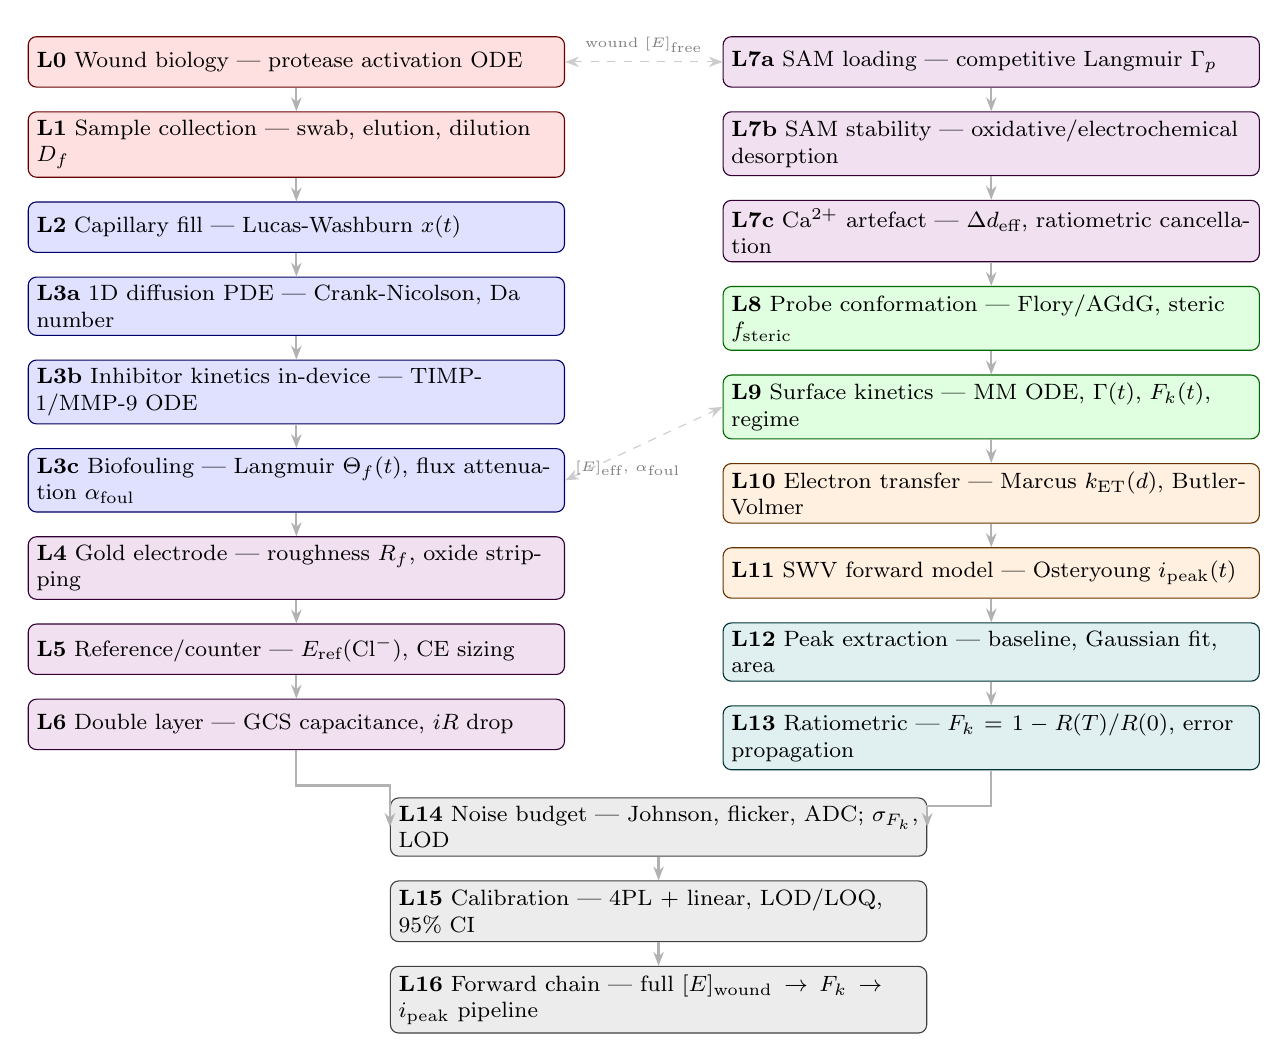
\begin{tikzpicture}[
  node distance=0.30cm and 1.0cm,
  lbox/.style={rectangle, rounded corners=3pt,
               minimum width=6.8cm, minimum height=0.64cm,
               text width=6.6cm, align=left, font=\footnotesize,
               inner sep=3pt},
  arr/.style={{Stealth[length=5pt]}-{Stealth[length=5pt]}, draw=gray!70},
  singlearr/.style={-{Stealth[length=5pt]}, thick, draw=gray!60},
  bio/.style    ={lbox, fill=red!12,    draw=red!40!black},
  trans/.style  ={lbox, fill=blue!12,   draw=blue!40!black},
  elec/.style   ={lbox, fill=violet!12, draw=violet!40!black},
  kin/.style    ={lbox, fill=green!12,  draw=green!40!black},
  swv/.style    ={lbox, fill=orange!12, draw=orange!40!black},
  sig/.style    ={lbox, fill=teal!12,   draw=teal!40!black},
  cal/.style    ={lbox, fill=gray!15,   draw=gray!50!black},
]

% ── Left column: Layers 0–8 ──────────────────────────────────────
\node[bio]   (L0) {\textbf{L0} Wound biology — protease activation ODE};
\node[bio,   below=of L0] (L1) {\textbf{L1} Sample collection — swab, elution, dilution $D_f$};
\node[trans, below=of L1] (L2) {\textbf{L2} Capillary fill — Lucas-Washburn $x(t)$};
\node[trans, below=of L2] (L3a){\textbf{L3a} 1D diffusion PDE — Crank-Nicolson, Da number};
\node[trans, below=of L3a](L3b){\textbf{L3b} Inhibitor kinetics in-device — TIMP-1/MMP-9 ODE};
\node[trans, below=of L3b](L3c){\textbf{L3c} Biofouling — Langmuir $\Theta_f(t)$, flux attenuation $\alpha_\text{foul}$};
\node[elec,  below=of L3c](L4) {\textbf{L4} Gold electrode — roughness $R_f$, oxide stripping};
\node[elec,  below=of L4] (L5) {\textbf{L5} Reference/counter — $E_\text{ref}(\text{Cl}^-)$, CE sizing};
\node[elec,  below=of L5] (L6) {\textbf{L6} Double layer — GCS capacitance, $iR$ drop};

% ── Right column: Layers 7–16 ────────────────────────────────────
\node[elec,  right=2.0cm of L0] (L7a){\textbf{L7a} SAM loading — competitive Langmuir $\Gamma_p$};
\node[elec,  below=of L7a](L7b){\textbf{L7b} SAM stability — oxidative/electrochemical desorption};
\node[elec,  below=of L7b](L7c){\textbf{L7c} Ca$^{2+}$ artefact — $\Delta d_\text{eff}$, ratiometric cancellation};
\node[kin,   below=of L7c](L8) {\textbf{L8} Probe conformation — Flory/AGdG, steric $f_\text{steric}$};
\node[kin,   below=of L8] (L9) {\textbf{L9} Surface kinetics — MM ODE, $\Gamma(t)$, $F_k(t)$, regime};
\node[swv,   below=of L9] (L10){\textbf{L10} Electron transfer — Marcus $k_\text{ET}(d)$, Butler-Volmer};
\node[swv,   below=of L10](L11){\textbf{L11} SWV forward model — Osteryoung $i_\text{peak}(t)$};
\node[sig,   below=of L11](L12){\textbf{L12} Peak extraction — baseline, Gaussian fit, area};
\node[sig,   below=of L12](L13){\textbf{L13} Ratiometric — $F_k = 1 - R(T)/R(0)$, error propagation};

% ── Bottom: Layers 14–16 (span both columns) ─────────────────────
\node[cal, below=0.6cm of L6, xshift=4.6cm] (L14){\textbf{L14} Noise budget — Johnson, flicker, ADC; $\sigma_{F_k}$, LOD};
\node[cal, below=of L14] (L15){\textbf{L15} Calibration — 4PL + linear, LOD/LOQ, 95\% CI};
\node[cal, below=of L15] (L16){\textbf{L16} Forward chain — full $[E]_\text{wound} \to F_k \to i_\text{peak}$ pipeline};

% ── Arrows left column ───────────────────────────────────────────
\foreach \a/\b in {L0/L1, L1/L2, L2/L3a, L3a/L3b, L3b/L3c, L3c/L4, L4/L5, L5/L6}
  \draw[singlearr] (\a.south) -- (\b.north);

% ── Arrows right column ──────────────────────────────────────────
\foreach \a/\b in {L7a/L7b, L7b/L7c, L7c/L8, L8/L9, L9/L10, L10/L11, L11/L12, L12/L13}
  \draw[singlearr] (\a.south) -- (\b.north);

% ── Cross-connections ────────────────────────────────────────────
\draw[singlearr] (L6.south) -- ++(0,-0.45) -| (L14.west);
\draw[singlearr] (L13.south) -- ++(0,-0.45) -| (L14.east);
\draw[singlearr] (L14.south) -- (L15.north);
\draw[singlearr] (L15.south) -- (L16.north);

% Layer 0→L7a coupling (SAM parameters from surface chemistry)
\draw[arr, gray!40, dashed] (L0.east) -- (L7a.west)
    node[midway, above, font=\tiny, text=gray]
    {wound $[E]_\text{free}$};
\draw[arr, gray!40, dashed] (L3c.east) -- (L9.west)
    node[midway, font=\tiny, text=gray, pos=0.4, below]
    {$[E]_\text{eff}$, $\alpha_\text{foul}$};

\end{tikzpicture}
\caption*{\small Colour key: {\color{red!60!black}\rule[0.4ex]{8pt}{5pt}} Biological/analytical \;
{\color{blue!60!black}\rule[0.4ex]{8pt}{5pt}} Transport \;
{\color{violet!60!black}\rule[0.4ex]{8pt}{5pt}} Electrode/SAM \;
{\color{green!60!black}\rule[0.4ex]{8pt}{5pt}} Surface kinetics \;
{\color{orange!60!black}\rule[0.4ex]{8pt}{5pt}} Electrochemistry \;
{\color{teal!60!black}\rule[0.4ex]{8pt}{5pt}} Signal processing \;
{\color{gray!70}\rule[0.4ex]{8pt}{5pt}} Calibration/output}
\end{figure}

%─────────────────────────────────────────────────────────────────
\begin{findingbox}
\textbf{Key computed results (all at $\alpha = 0.3$, C15 substrate, $T = 30$ min unless stated).}
\begin{itemize}[noitemsep,topsep=0pt]
\item $F_k$ at 17 ng/mL: \textbf{1.0\%} at 30 min, \textbf{2.0\%} at 60 min (below 5\% threshold; see regime analysis)
\item $F_k$ at 200 ng/mL: \textbf{11.4\%} at 30 min, \textbf{21.9\%} at 60 min
\item No valid linear calibration window at $\alpha = 0.3$ (detect $>82$ min; linear $<51$ min) $\to$ use 4PL calibration or increase $\alpha$
\item Electronic noise floor (Johnson + ADC): $\sigma_i = 0.088$ pA; $\sigma_{F_k} = 0.003\%$ --- electronics are NOT the limiting factor
\item Kinetic LOD $= 8.8$ ng/mL at $T = 30$ min (3$\sigma$/slope); LOQ $= 29.4$ ng/mL --- below 17 ng/mL clinical lower bound $\checkmark$
\item TIMP-1 strongly suppresses MMP-9 in device: at 200 ng/mL TIMP-1 chamber concentration, $>$70\% of MMP-9 is inhibited within 30 min
\item C15 substrate selected over A11: F$_k$(17 ng/mL, $\alpha$=1, 60 min) = 11.8\% vs 4.4\%; $\Delta F_k$ = 65.3\% vs 34.8\%
\end{itemize}
\end{findingbox}

%─────────────────────────────────────────────────────────────────
\section{Layer 0: Wound Biology --- Protease Activation Cascade}

The free enzyme concentrations entering the device are set by the wound biochemistry. The full activation cascade ODE integrates pro-enzyme activation, inhibitor binding, and complex formation simultaneously.

\begin{eqbox}
\textbf{MMP-9 cascade} (9-state ODE):
$\frac{d[\text{proMMP-9}]}{dt} = -(k_{\text{cat}}/K_m)_{\text{MMP-3}} [\text{MMP-3}][\text{proMMP-9}]
    - (k_{\text{cat}}/K_m)_{\text{plasmin}}[\text{plasmin}][\text{proMMP-9}]$\\
$\frac{d[\text{MMP-9}]}{dt} = \text{activation} - k_{\text{on,T1}}[\text{TIMP-1}][\text{MMP-9}] + k_{\text{off,T1}}[\text{MMP-9:TIMP-1}]$\\[0.3em]
\textbf{HNE cascade:}
$\frac{d[\text{HNE}]}{dt} = -k_{\text{on,A1AT}}[\text{A1AT}][\text{HNE}] - k_{\text{on,SLPI}}[\text{SLPI}][\text{HNE}]$
\end{eqbox}

\noindent\textbf{Confident values:} $k_{\text{on,A1AT}} = 2\times10^7$ M$^{-1}$s$^{-1}$ (Beatty 1980; Bieth 1984);
$K_i(\text{TIMP-1/MMP-9}) \approx 0.1$ nM (Nagase \& Woessner 1999);
$[\text{Cl}^-]_\text{wound} = 150$ mM; $E^\circ_\text{AgCl} = 0.2224$ V vs SHE (Bard \& Faulkner).

\noindent\flagged{$(k_\text{cat}/K_m)_\text{MMP-3}$, $(k_\text{cat}/K_m)_\text{plasmin}$, $k_{\text{on,TIMP-1}}$,
$k_{\text{on,SLPI}}$, $[\text{MMP-3}]_\text{wound}$, $[\text{plasmin}]_\text{wound}$,
$[\text{A1AT}]_\text{wound}$, $[\text{SLPI}]_\text{wound}$, $[\text{TIMP-1}]_\text{wound}$ free fraction.}

\begin{figure}[H]
\centering
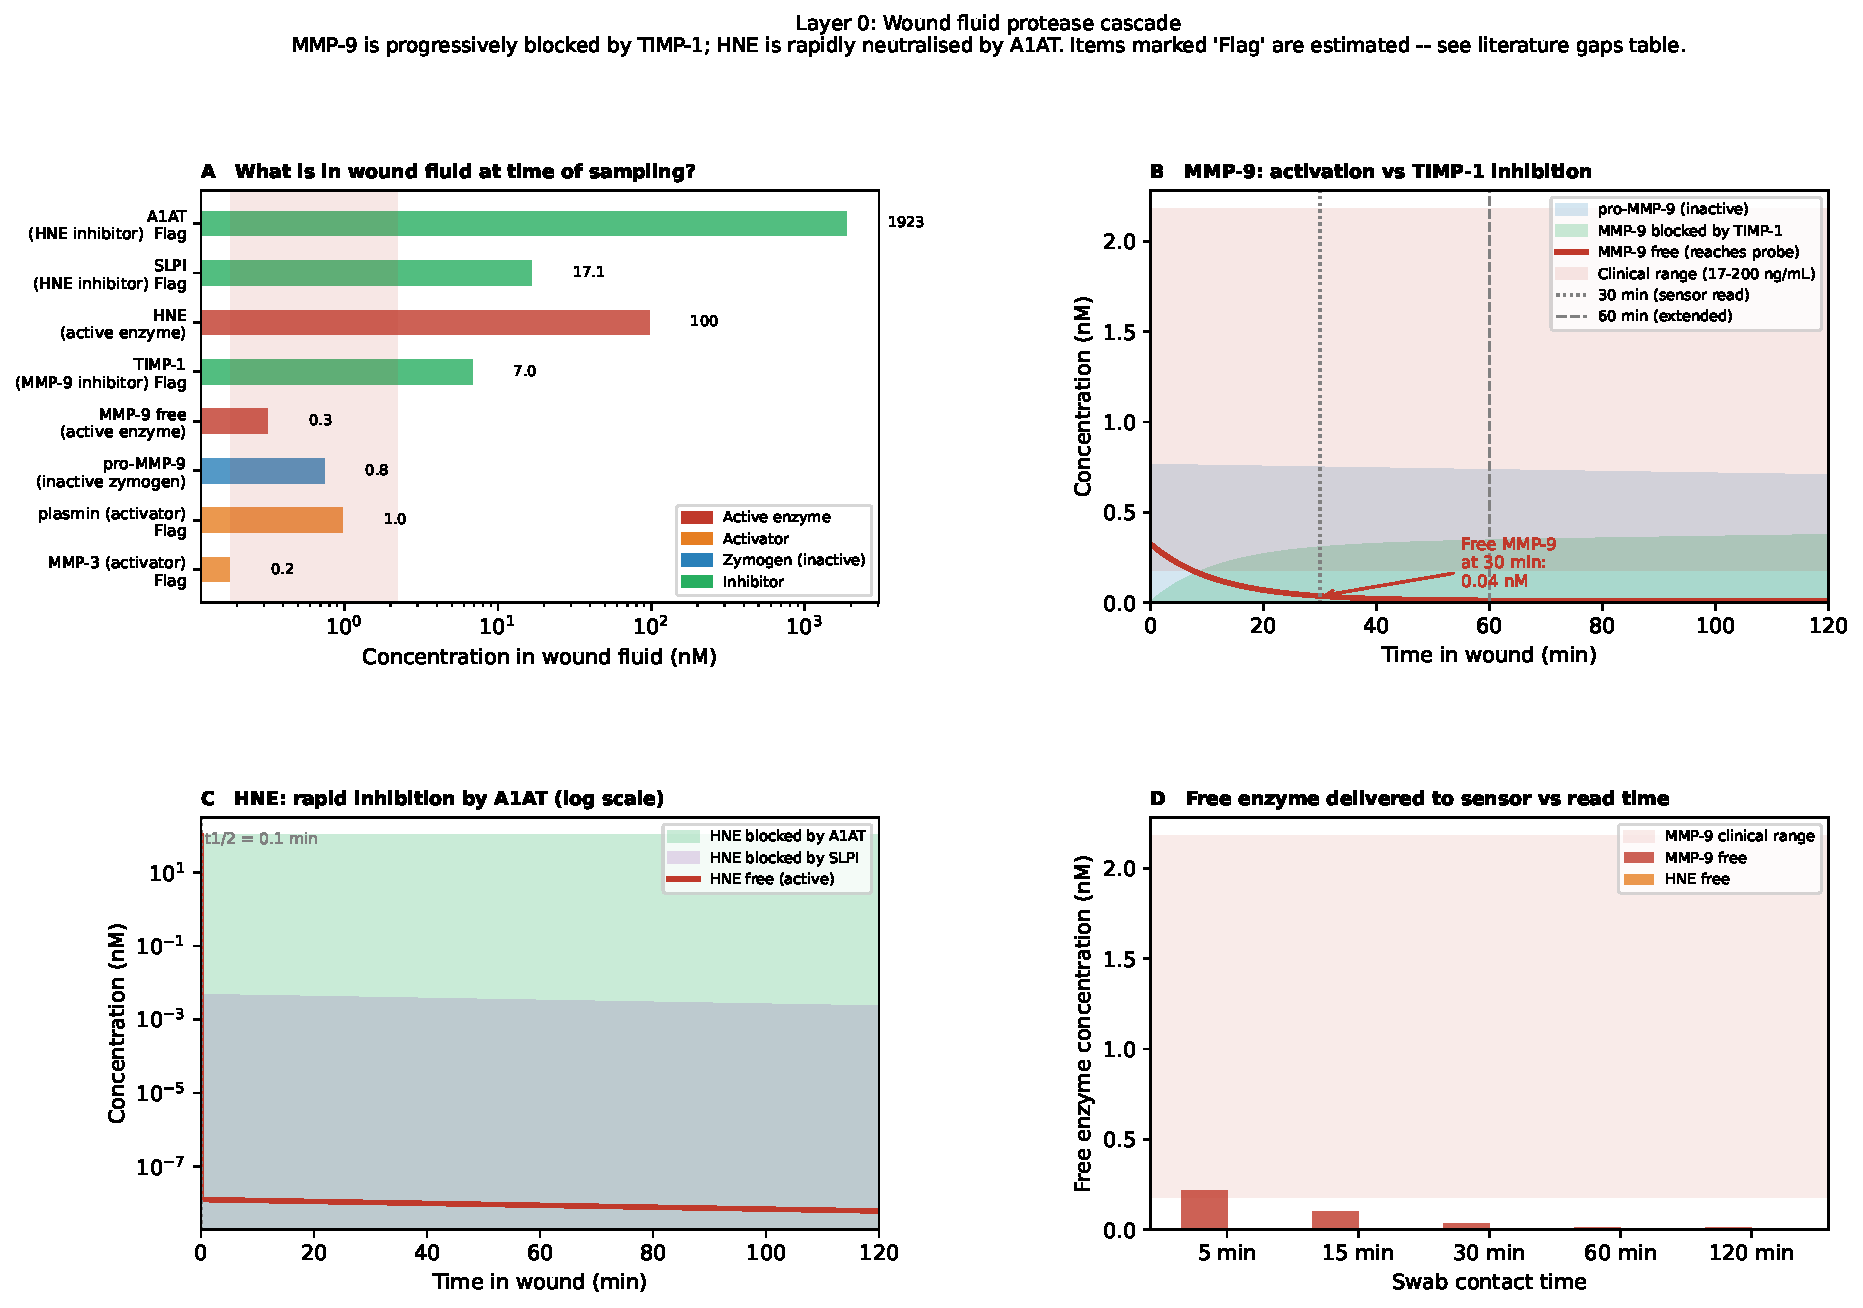
\includegraphics[width=\linewidth]{figures/fig_B1_wound_biology.pdf}
\caption{Layer 0 output: wound-fluid protease cascade ODE. Panel D shows the free enzyme concentrations
input to Layer 1. Shaded region = swab contact window. Note rapid TIMP-1-mediated MMP-9 inhibition.}
\end{figure}

%─────────────────────────────────────────────────────────────────
\section{Layer 1: Sample Collection}

Swab absorption ($V_\text{abs} = 30\,\mu$L), elution into buffer ($V_\text{elut} = 60\,\mu$L, $D_f = 2$):
\begin{equation}
[E]_\text{chamber} = [E]_\text{wound} \times \eta_\text{elut} / D_f
\end{equation}
SLPI (11.7 kDa, $\eta = 0.85$) elutes more efficiently than HNE (30 kDa, $\eta = 0.75$), increasing the SLPI:HNE inhibitor ratio in the chamber (enrichment factor 1.13$\times$).

\flagged{All species-specific elution efficiencies $\eta$ except SLPI (Ashcroft 2000) and GSH/ascorbate. Validate with swab recovery assay.}

\begin{figure}[H]
\centering
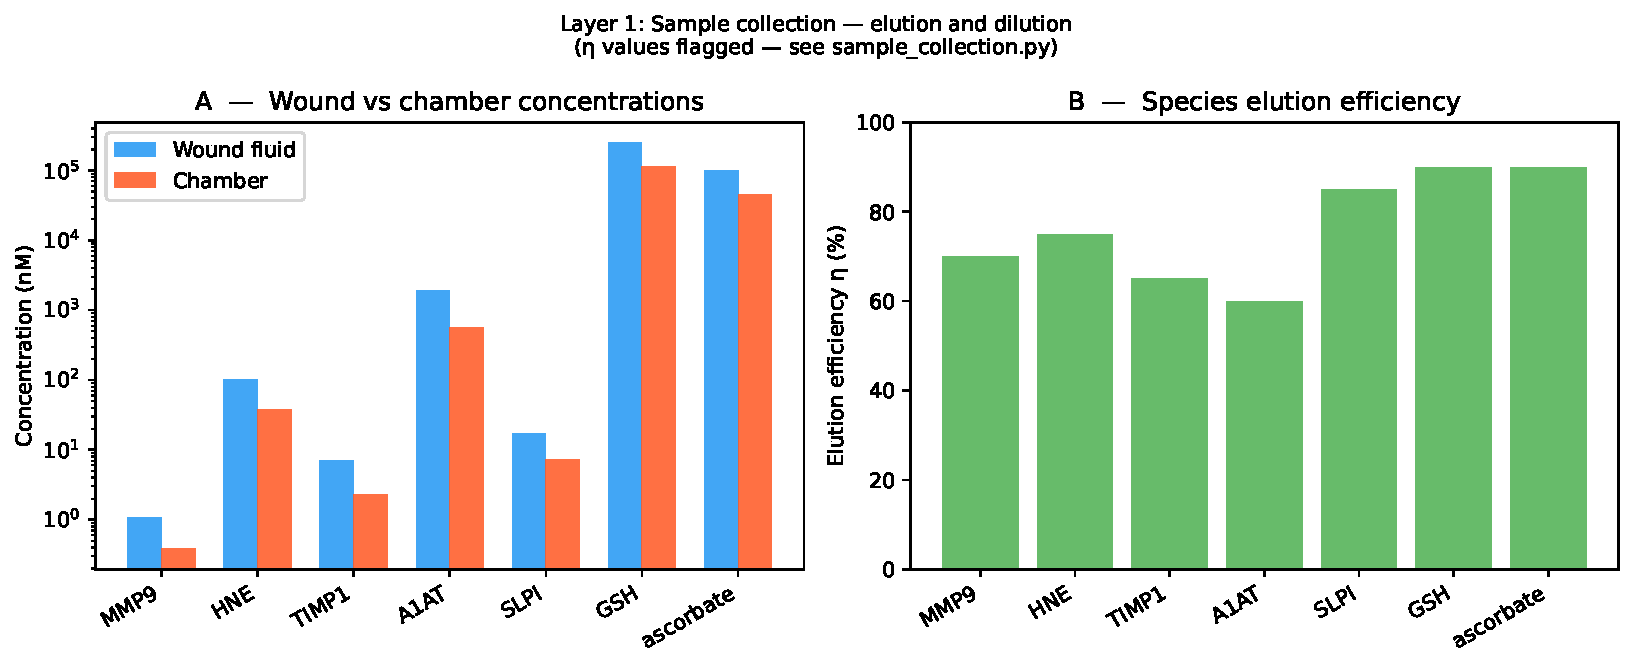
\includegraphics[width=0.85\linewidth]{figures/fig_B1b_sample_collection.pdf}
\caption{Layer 1: Wound vs chamber concentrations (log scale) and elution efficiency $\eta$ per species.
MMP-9 undergoes 2.86$\times$ dilution (D$_f = 2$, $\eta = 0.70$). All $\eta$ values are flagged.}
\end{figure}

%─────────────────────────────────────────────────────────────────
\section{Layer 2: Capillary Fill}

Lucas-Washburn for rectangular channel ($w \times h$ cross-section):
\begin{equation}
x(t) = \sqrt{\frac{r_h \gamma \cos\theta}{2\eta_\text{fluid}} \cdot t}, \qquad
r_h = \frac{2wh}{w+h}
\end{equation}
Fill time is fast ($\ll$1 min for 20 mm channel), so all electrodes are wetted well before the incubation window. Damk\"{o}hler number Da $\approx 556 \gg 1$ --- enzyme transport to the electrode is \textit{not} rate-limiting; kinetics dominate.

\flagged{Contact angle $\theta = 30^\circ$ (assumed; measure on actual chip surface)}

\begin{figure}[H]
\centering
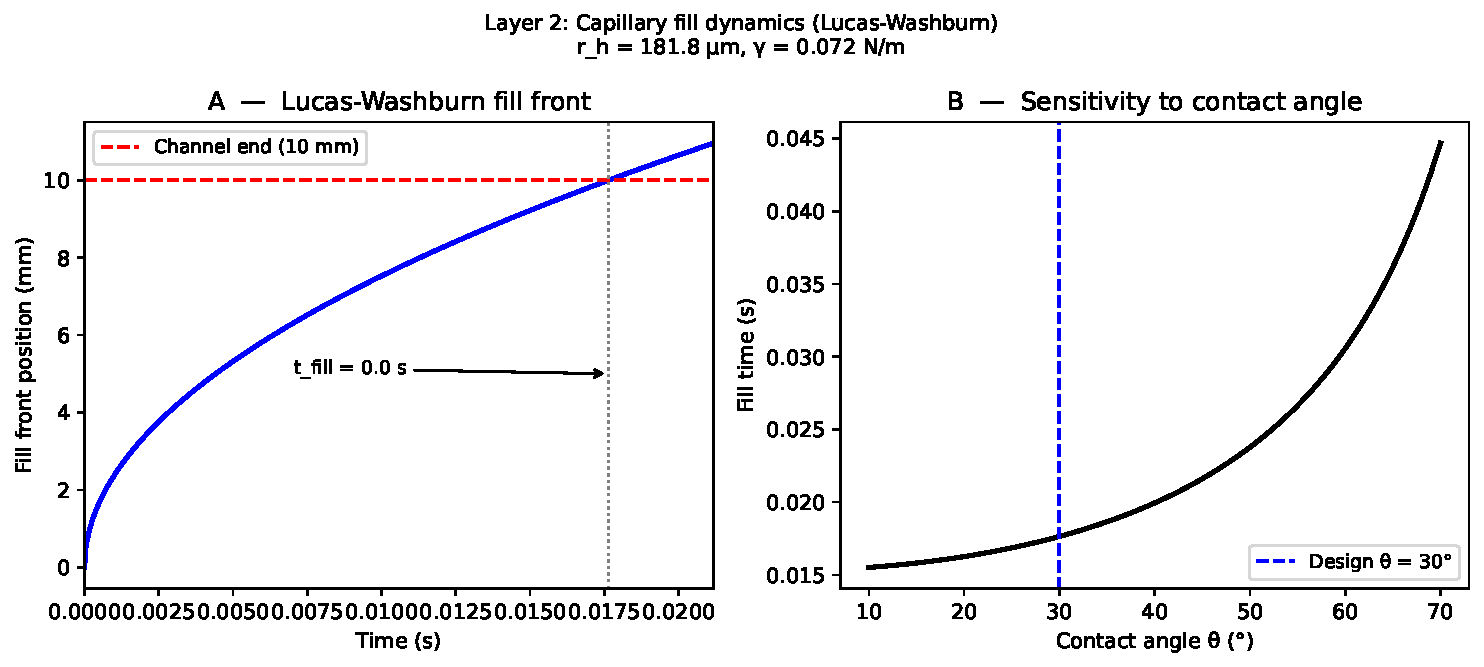
\includegraphics[width=\linewidth]{figures/fig_B2_capillary_fill.pdf}
\caption{Layer 2: Lucas-Washburn fill dynamics. Channel fills completely in $<$0.2 s with $\theta = 30^\circ$.
Panel C: Damk\"{o}hler number vs $[E]$ confirms kinetic-limited regime (Da $\gg 1$).}
\end{figure}

%─────────────────────────────────────────────────────────────────
\section{Layers 3a--3c: Mass Transport, Fouling, and Inhibitor Kinetics}

\subsection{3a: Diffusion PDE (Crank-Nicolson)}

1D diffusion equation with Robin boundary condition at the electrode:
\begin{align}
\frac{\partial [E]}{\partial t} &= D_E \frac{\partial^2 [E]}{\partial z^2}, \quad z \in (0, h)\\
D_E \frac{\partial [E]}{\partial z}\bigg|_{z=0} &= k_\text{obs}[E](0,t)\,\Gamma
\end{align}
$D_\text{MMP-9} = 4.7\times10^{-11}$ m$^2$s$^{-1}$ (Stokes-Einstein, $r = 3.5$ nm). The Crank-Nicolson scheme ensures stability for all time-steps.

\begin{figure}[H]
\centering
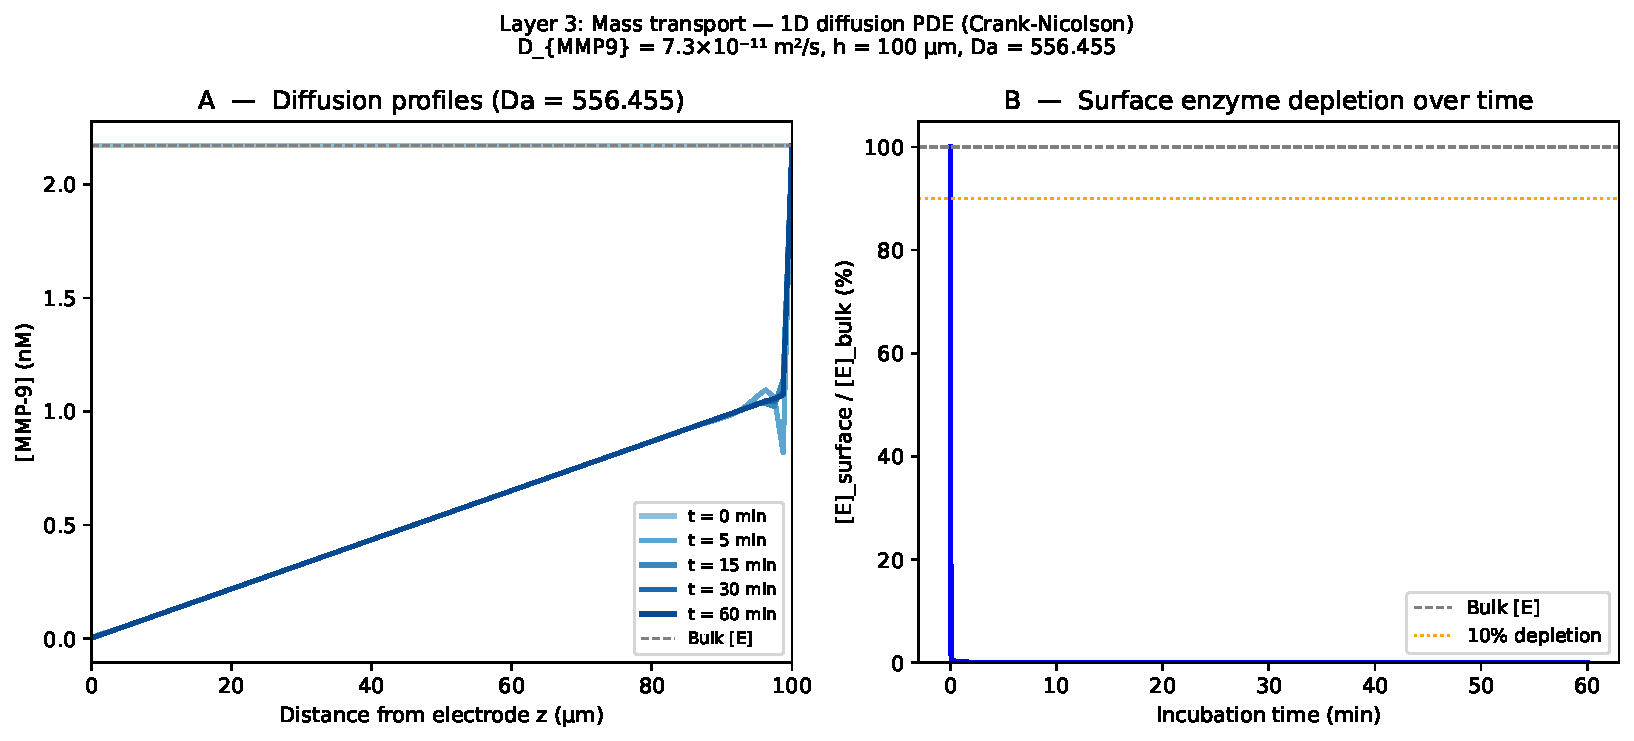
\includegraphics[width=\linewidth]{figures/fig_B3_mass_transport.pdf}
\caption{Layer 3a: 1D diffusion of MMP-9 to the electrode surface. Enzyme is not depleted at the surface
in the clinical range (Da $\ll 1$ in kinetic terms) --- [E] remains approximately uniform.}
\end{figure}

\subsection{3c: Biofouling Attenuation}

Non-specific protein adsorption forms a layer of thickness $h_f$ that attenuates enzyme flux:
\begin{equation}
\frac{d\Theta_f}{dt} = k_f [P]_\text{bulk}(1 - \Theta_f) - k_d \Theta_f, \qquad
\alpha_\text{foul}(t) = \frac{h_\text{channel}}{h_\text{channel} + h_{f,\text{max}} \Theta_f}
\end{equation}

\flagged{$k_f = 10^3$ M$^{-1}$s$^{-1}$, $k_d = 10^{-4}$ s$^{-1}$, $P_\text{bulk} = 150\,\mu$M (total protein)}

\begin{figure}[H]
\centering
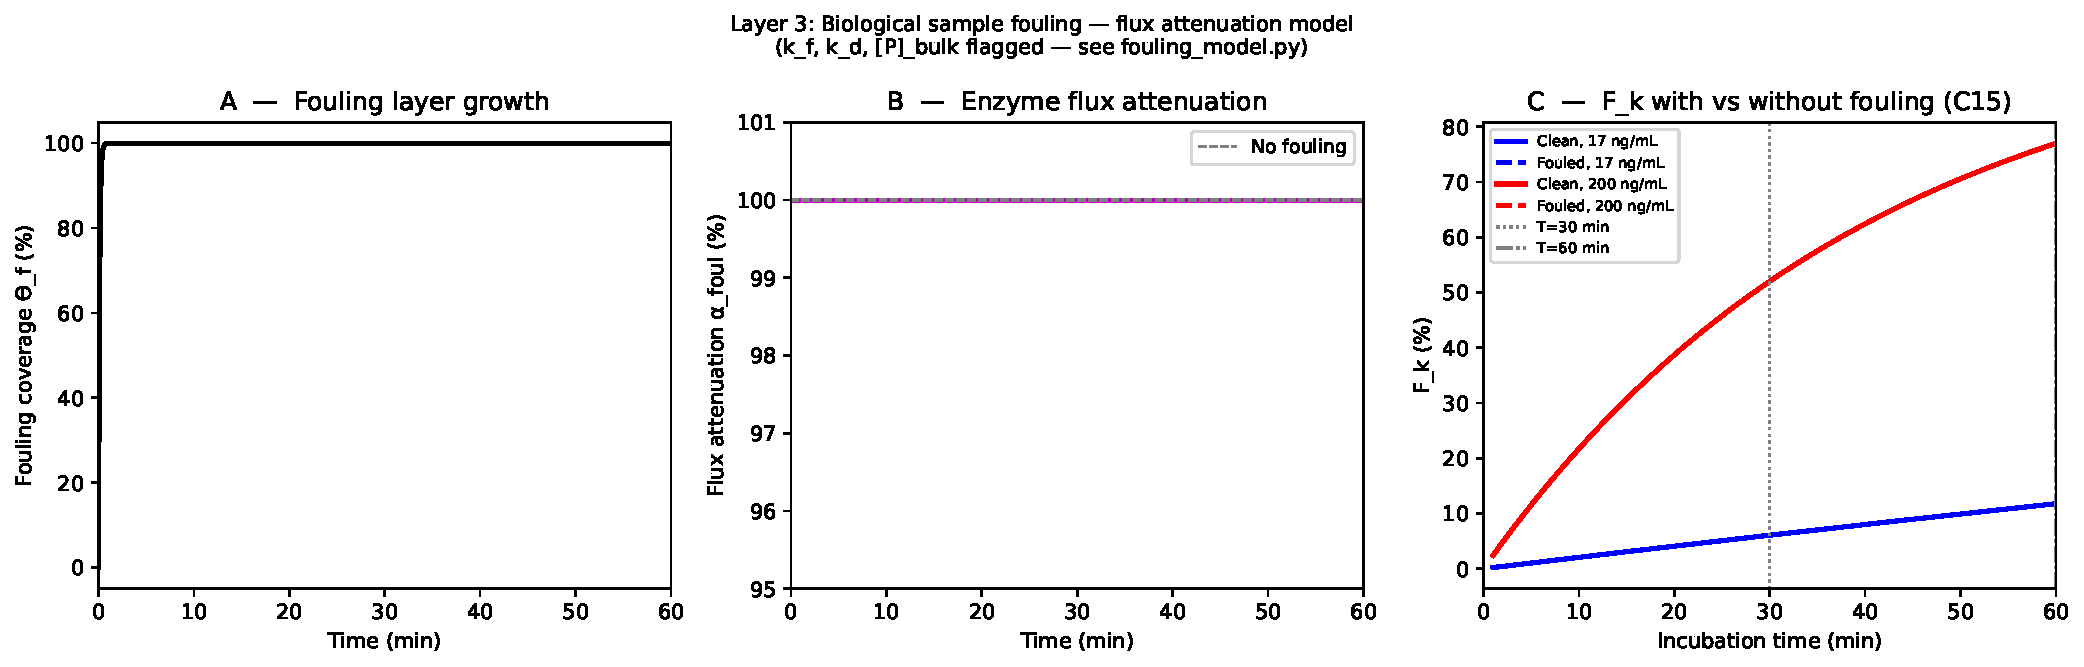
\includegraphics[width=\linewidth]{figures/fig_B4_fouling.pdf}
\caption{Layer 3c: Biofouling coverage $\Theta_f(t)$ and its flux attenuation $\alpha_\text{foul}$.
The fouling layer saturates rapidly but its net effect on $F_k$ is minimal ($<$0.01\%) because
$h_f \ll h_\text{channel}$. Flagged parameters dominate this layer's uncertainty.}
\end{figure}

\subsection{3b: In-Device Inhibitor Kinetics}

After fill, TIMP-1 co-eluted from wound fluid continues to inhibit MMP-9 in solution:
\begin{equation}
\frac{d[E]_\text{free}}{dt} = -k_{\text{on,T1}}[E]_\text{free}[I]_\text{free} + k_{\text{off,T1}}[EI]
\end{equation}
At TIMP-1 chamber concentration $\approx 2.3$ nM vs MMP-9 $\approx 0.06$ nM (at 17 ng/mL after dilution), TIMP-1 is in large excess --- MMP-9 inhibition is nearly complete within 30 min.

\begin{figure}[H]
\centering
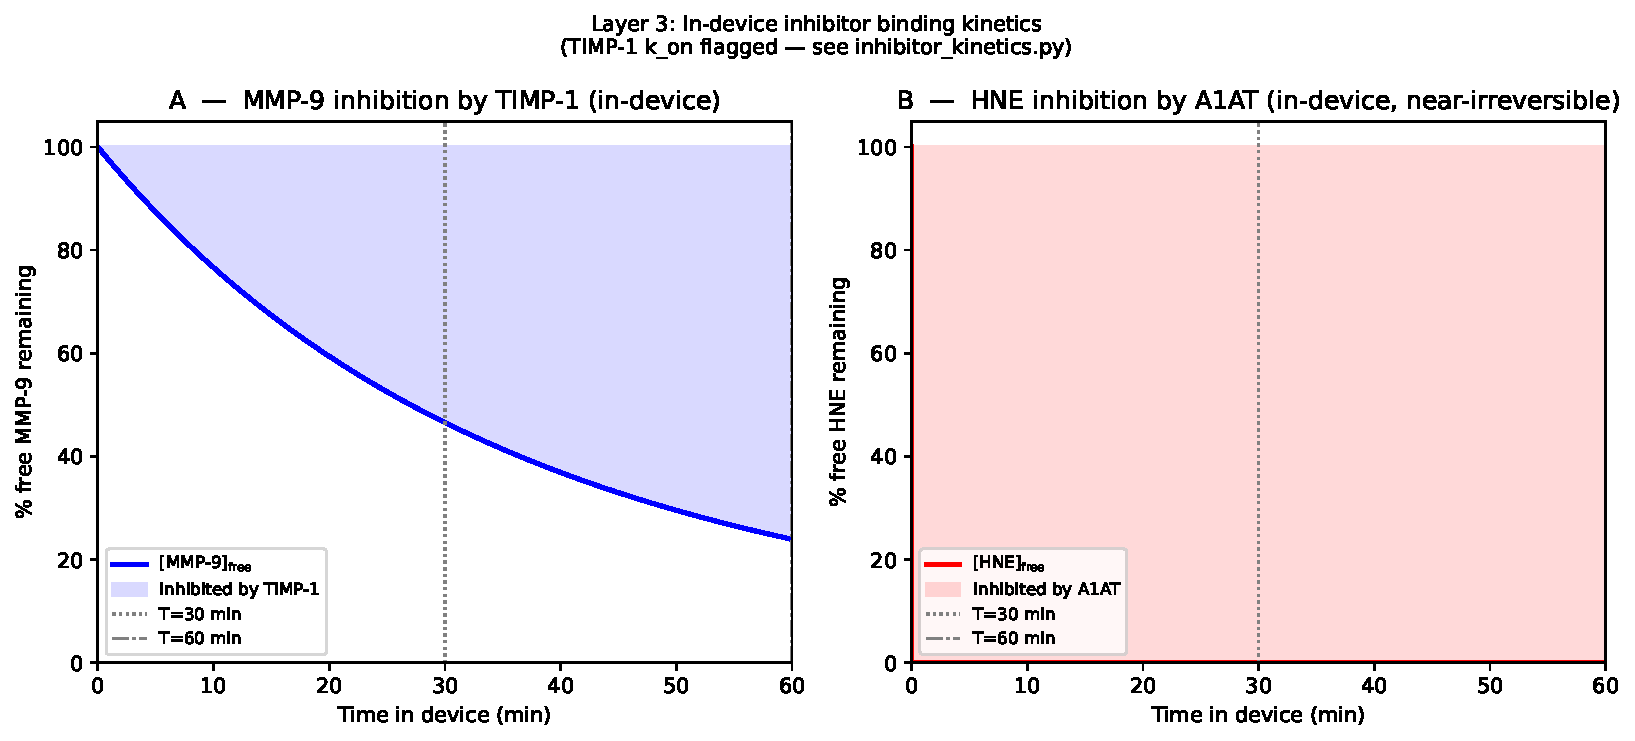
\includegraphics[width=\linewidth]{figures/fig_B5_inhibitor_kinetics.pdf}
\caption{Layer 3b: In-device inhibitor binding. At clinical MMP-9 concentrations, $>$70\% of MMP-9 is
complexed with TIMP-1 within 30 min. Free HNE is rapidly quenched by A1AT ($t_{1/2} \ll 1$ s).
This inhibitor depletion is the dominant factor limiting $F_k$ in the forward chain.}
\end{figure}

%─────────────────────────────────────────────────────────────────
\section{Layers 4--7: Electrode Surface and SAM Chemistry}

\subsection{Layer 4: Gold Electrode}

True electrode area: $A_\text{true} = R_f \times A_\text{geo}$, measured from Au oxide stripping charge:
$R_f = Q_\text{strip} / (Q_\text{ref} \times A_\text{geo})$, where \confident{$Q_\text{ref} = 390\,\mu$C\,cm$^{-2}$ (Trasatti \& Petrii 1992)}.

\flagged{$R_f = 1.5$ nominal; WE diameter 1.5 mm nominal --- must be confirmed by CV characterisation.}

\begin{figure}[H]
\centering
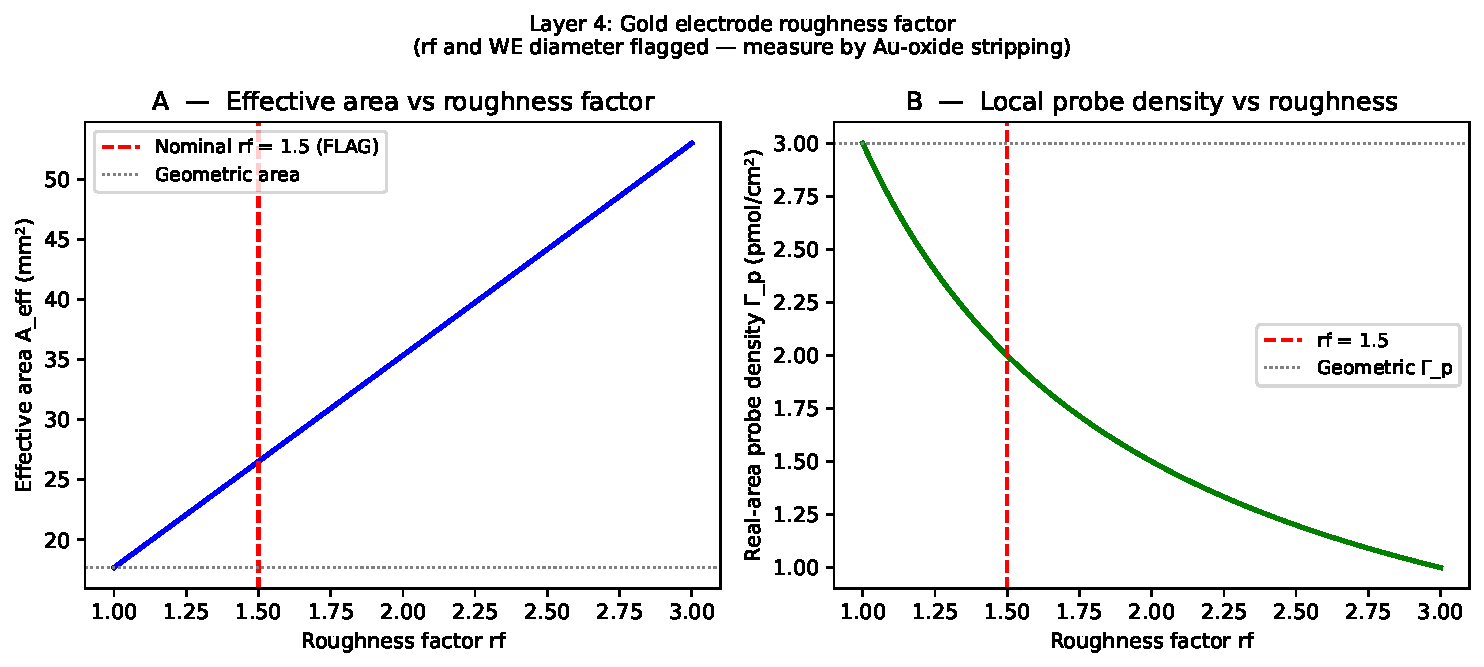
\includegraphics[width=\linewidth]{figures/fig_L4_gold_electrode.pdf}
\caption{Layer 4: Roughness factor calculation and effective area vs $Q_\text{oxide}$.}
\end{figure}

\subsection{Layer 5: Reference Electrode}

On-chip Ag/AgCl reference: $E_\text{ref} = E^\circ_\text{AgCl} - (RT/F)\ln([\text{Cl}^-])$.
\confident{$E^\circ_\text{AgCl} = 0.2224$ V vs SHE}, $[\text{Cl}^-]_\text{wound} = 150$ mM.
Wound-to-chamber Cl$^-$ shift produces $\Delta E_\text{ref} = 1.5$ mV --- negligible.

\begin{figure}[H]
\centering
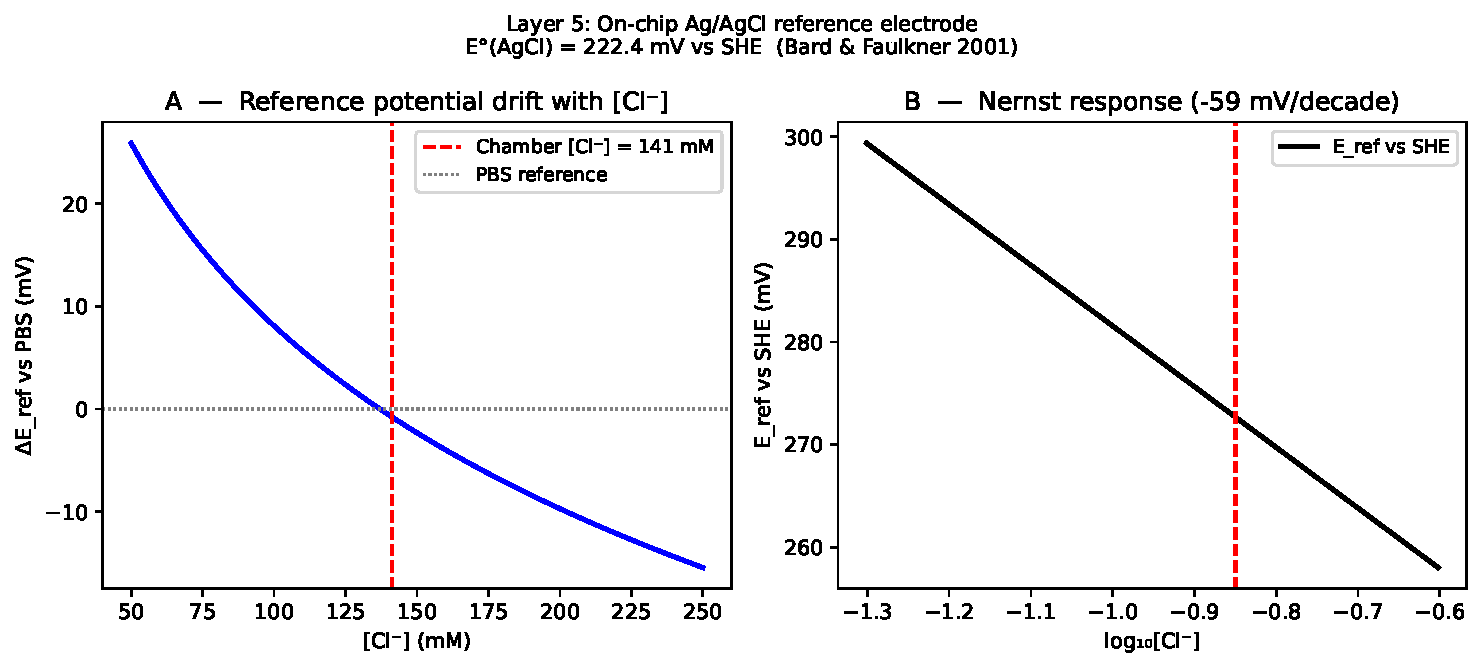
\includegraphics[width=\linewidth]{figures/fig_L5_reference.pdf}
\caption{Layer 5: Reference electrode potential vs Cl$^-$ concentration. Grey band = wound-fluid range.
Reference shift from wound to chamber is $<$2 mV --- within acceptable drift budget.}
\end{figure}

\subsection{Layer 6: Double Layer}

Gouy-Chapman-Stern model: $C_\text{dl}^{-1} = C_H^{-1} + C_\text{GC}^{-1}$.
At 163 mM ionic strength (PBS), the Gouy-Chapman capacitance $C_\text{GC}$ is large --- $C_\text{dl}$ is dominated by the Helmholtz layer.
Double-layer charging current in SWV: $I_\text{cap} = 2C_\text{dl}A\Delta E_\text{SW} f \approx 0.6$ nA (far below the faradaic MB peak).

\flagged{$C_H = 30\,\mu$F\,cm$^{-2}$ (MCH-SAM --- measure by EIS)}

\begin{figure}[H]
\centering
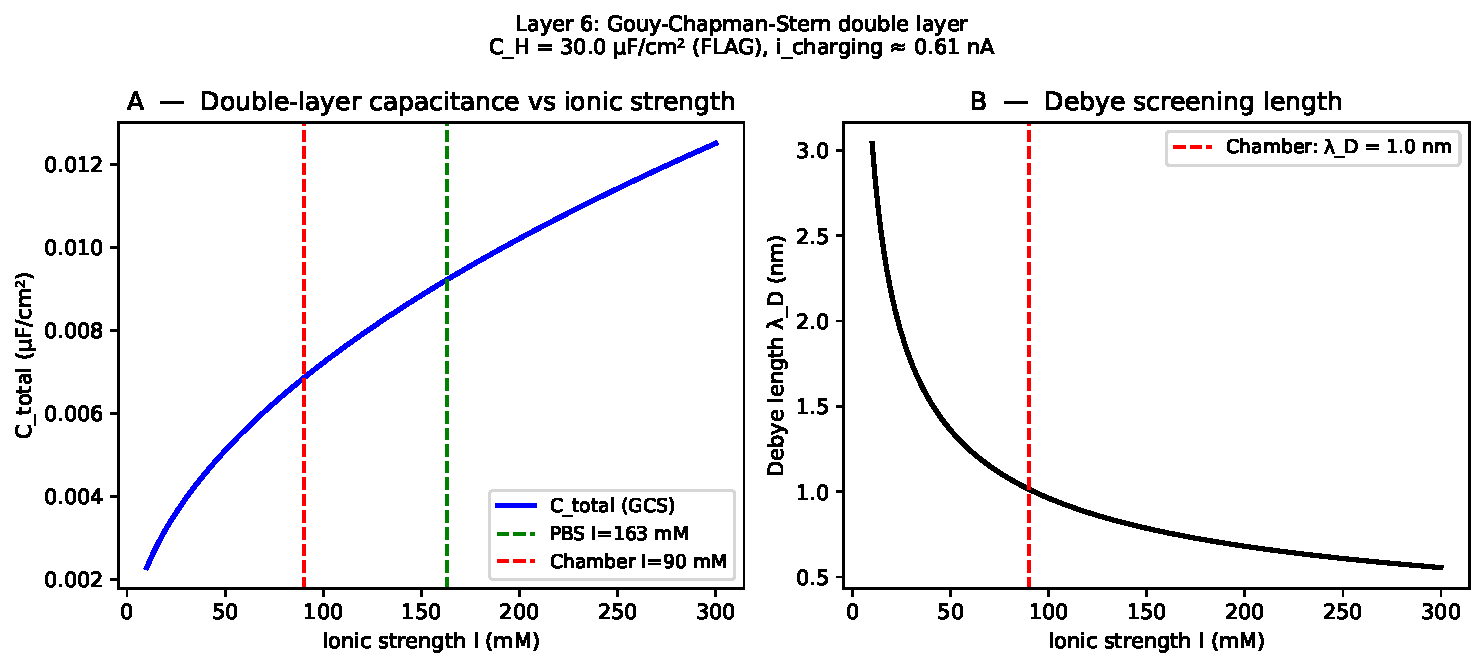
\includegraphics[width=\linewidth]{figures/fig_L6_double_layer.pdf}
\caption{Layer 6: Double-layer capacitance model. Total $C_\text{dl}$ and charging current are well below
the faradaic limit across all ionic strengths encountered.}
\end{figure}

\subsection{Layer 7: SAM Formation and Stability}

Probe surface density from competitive Langmuir adsorption:
\begin{equation}
\frac{\Gamma_p}{\Gamma_\text{max}} = \frac{K_{a,p} c_p}{1 + K_{a,p} c_p + K_{a,d} c_d}
\end{equation}
Target $\Gamma_p = 2$--$3$ pmol\,cm$^{-2}$ to avoid complete steric blocking (see Layer 8). Achieve with $c_p \approx 6\,\mu$M probe and $c_d = 100\,\mu$M MCH.

\flagged{$K_{a,p}$, $K_{a,d}$ (adsorption constants for probe/MCH on Au in ethanol --- must measure)}

SAM stability: electrochemical desorption is safe (scan minimum $-0.65$ V vs $E_\text{des} = -0.90$ V, margin = 250 mV). Oxidative SAM loss at $[\text{H}_2\text{O}_2] = 10\,\mu$M, 60 min: 3.5\% --- acceptable.

\begin{figure}[H]
\centering
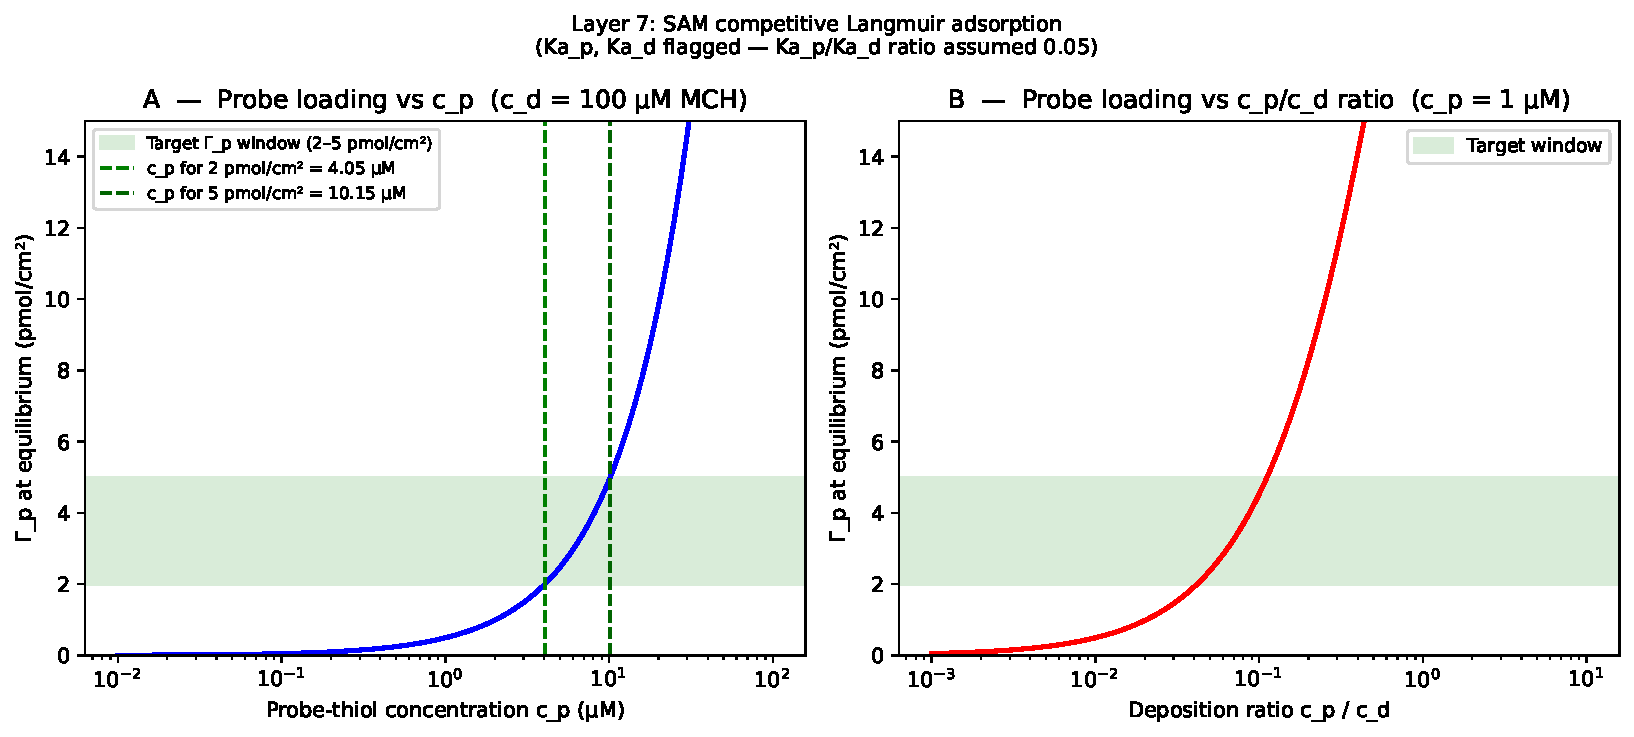
\includegraphics[width=0.9\linewidth]{figures/fig_B6_sam_loading.pdf}
\caption{Layer 7a: SAM loading. Panel A: $\Gamma_p$ vs probe concentration for several MCH concentrations.
Panel B: Diluent enrichment at surface (probe-poor surface relative to solution). Required solution
composition to hit $\Gamma_p = 3$ pmol\,cm$^{-2}$: $c_p \approx 6\,\mu$M (flagged Ka values).}
\end{figure}

\begin{figure}[H]
\centering
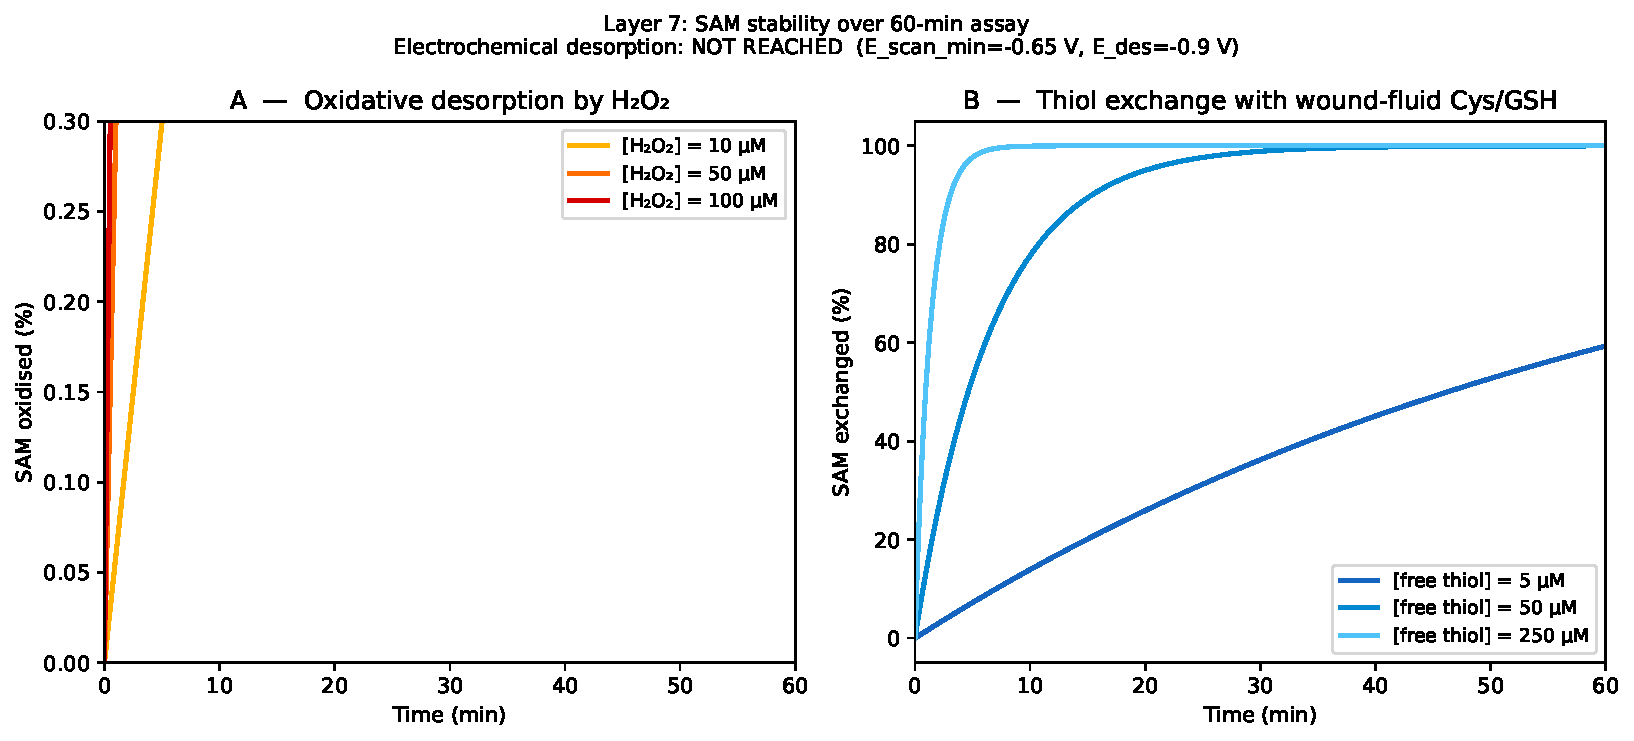
\includegraphics[width=0.9\linewidth]{figures/fig_L7b_sam_stability.pdf}
\caption{Layer 7b: SAM stability. Electrochemical desorption threshold $E_\text{des} = -0.90$ V vs
Ag/AgCl; operating minimum $-0.65$ V gives 250 mV safety margin. Oxidative loss at 10 $\mu$M
H$_2$O$_2$ over 60 min $\approx$ 3.5\% --- acceptable for 30--60 min assay window.}
\end{figure}

\begin{figure}[H]
\centering
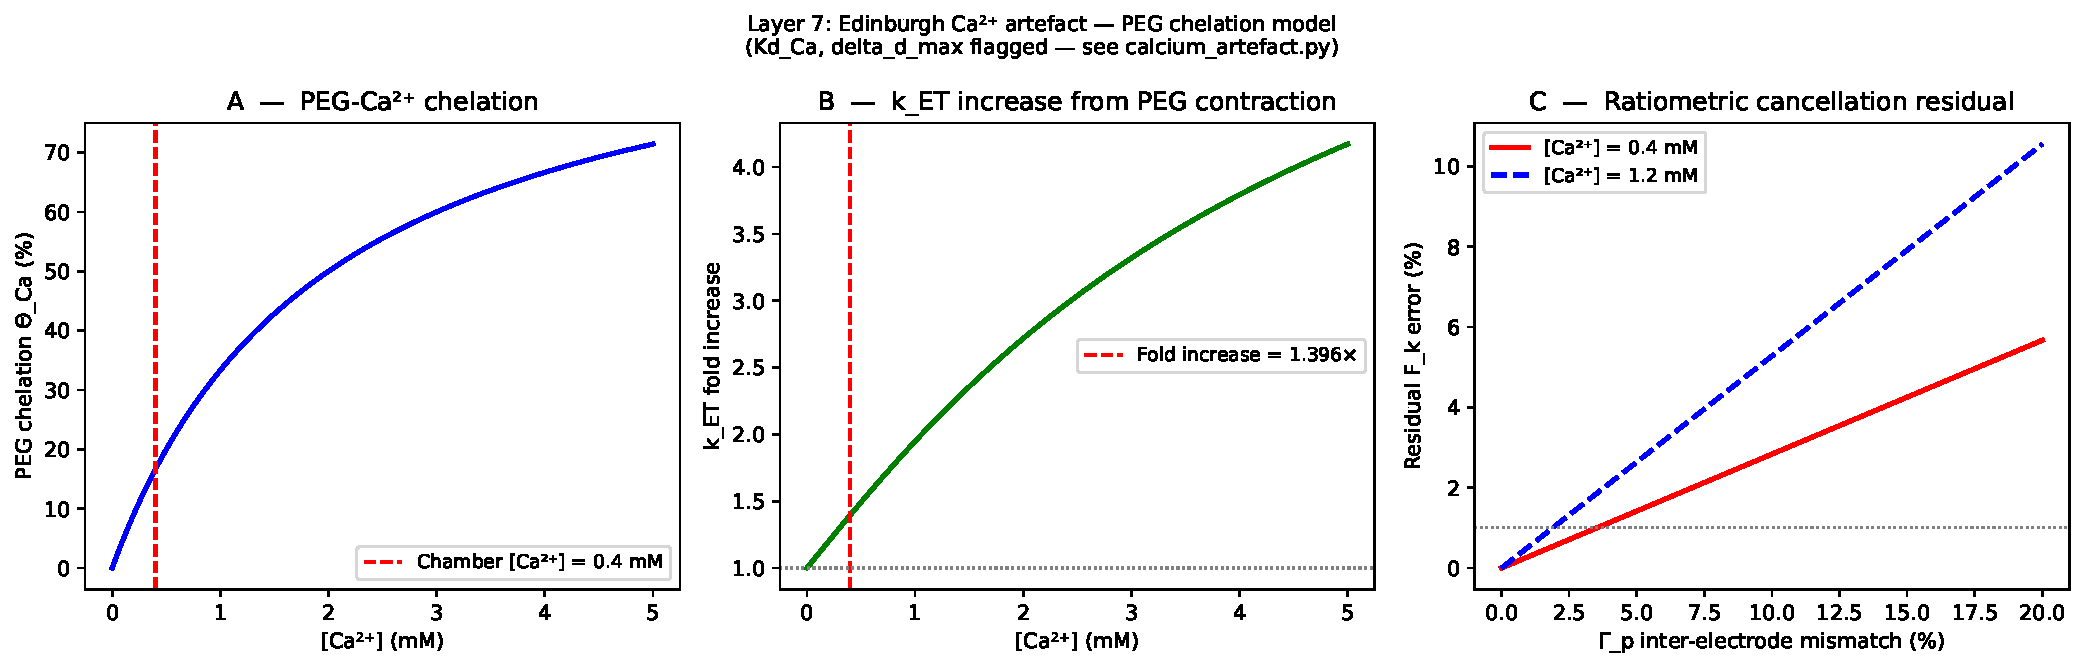
\includegraphics[width=0.9\linewidth]{figures/fig_L7c_calcium.pdf}
\caption{Layer 7c: Ca$^{2+}$ artefact. PEG chelates Ca$^{2+}$ ($K_d = 2$ mM, flagged), contracting the
tether by $\Delta d_\text{max}$ and increasing $k_\text{ET}$. Critically, the ratiometric design
cancels this artefact provided both active and control electrodes have identical $\Gamma_p$.}
\end{figure}

%─────────────────────────────────────────────────────────────────
\section{Layer 8: Probe Conformation and Steric Hindrance}

PEG$_6$ spacer conformation from Flory scaling (dilute regime) and Alexander-de Gennes (brush regime).
The MB-to-Au effective distance:
$d_\text{eff} = L_\text{PEG} + L_\text{peptide} + L_\text{MB} \approx 4.9$ nm.

Steric blocking by MMP-9 (radius $r = 4$ nm, PDB 1L6J):
\begin{equation}
\Gamma_\text{steric,max} = \frac{1}{\pi r_E^2 N_A} \approx 3.3\,\text{pmol\,cm}^{-2}
\end{equation}
At $\Gamma_p = 3$ pmol\,cm$^{-2}$, the accessibility factor $f_\text{steric} = 1 - \Gamma_p/\Gamma_\text{steric,max} = 0.09$ (9\%). This severely limits the effective surface kinetic rate.

\begin{findingbox}
\textbf{Design implication:} $\Gamma_p$ must be $< 3.3$ pmol\,cm$^{-2}$ or MMP-9 cannot physically access most probes. Target $\Gamma_p \leq 2$ pmol\,cm$^{-2}$ to maintain $f_\text{steric} > 40\%$.
\end{findingbox}

\begin{figure}[H]
\centering
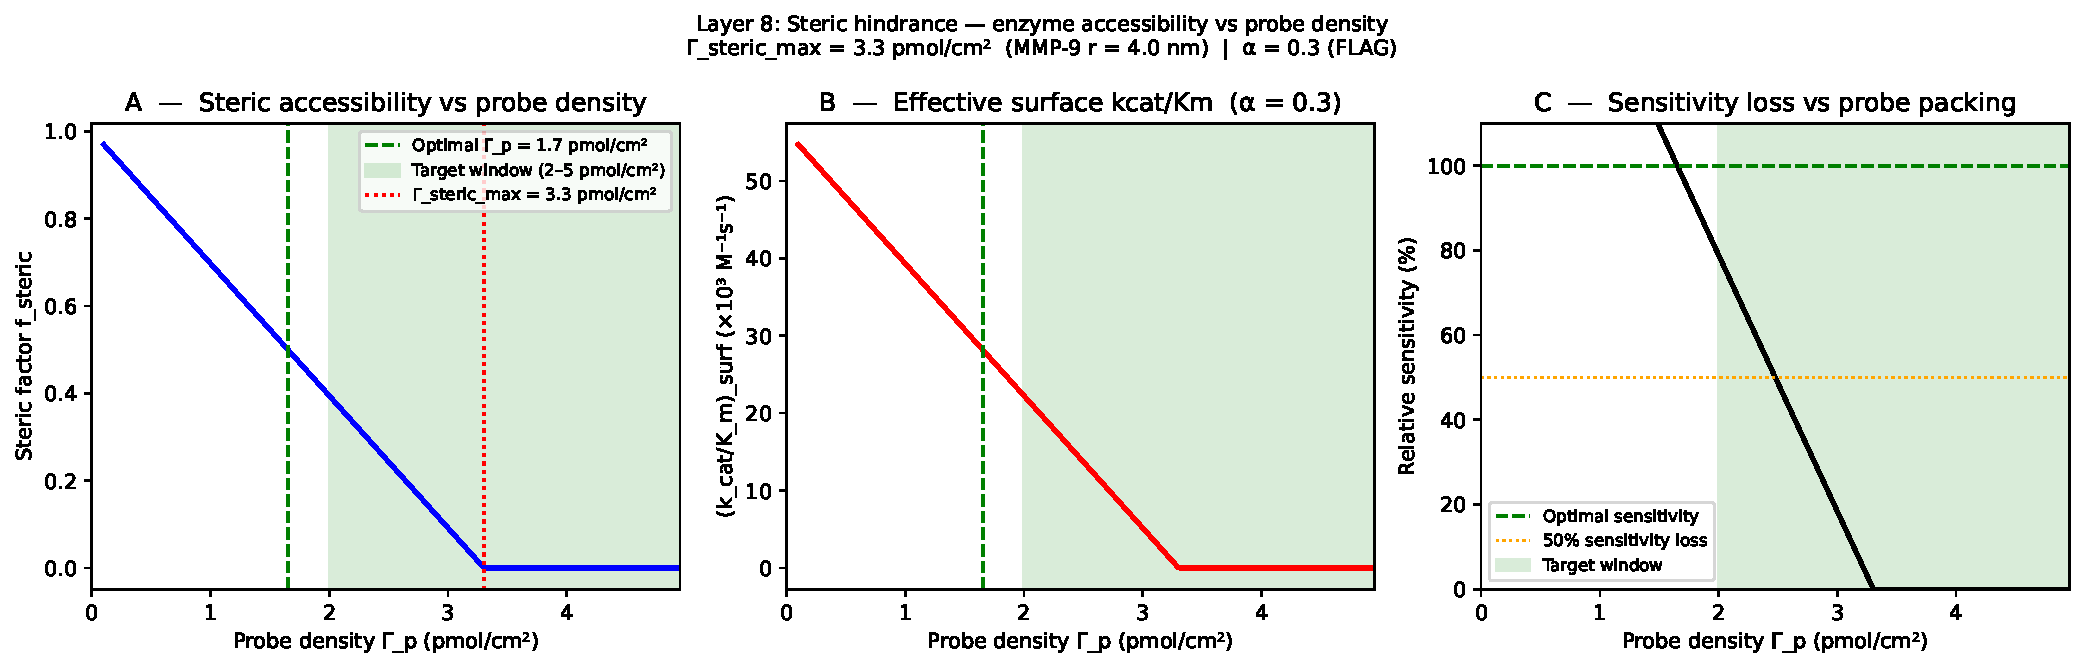
\includegraphics[width=\linewidth]{figures/fig_B7_steric_hindrance.pdf}
\caption{Layer 8: Steric hindrance factor $f_\text{steric}$ vs probe density $\Gamma_p$.
At 3 pmol/cm$^2$, only 9\% of probes are accessible to MMP-9. Relative sensitivity drops to 23\%.
At 5 pmol/cm$^2$, complete steric blocking ($f_\text{steric} = 0$): enzyme cannot reach substrate.}
\end{figure}

\begin{figure}[H]
\centering
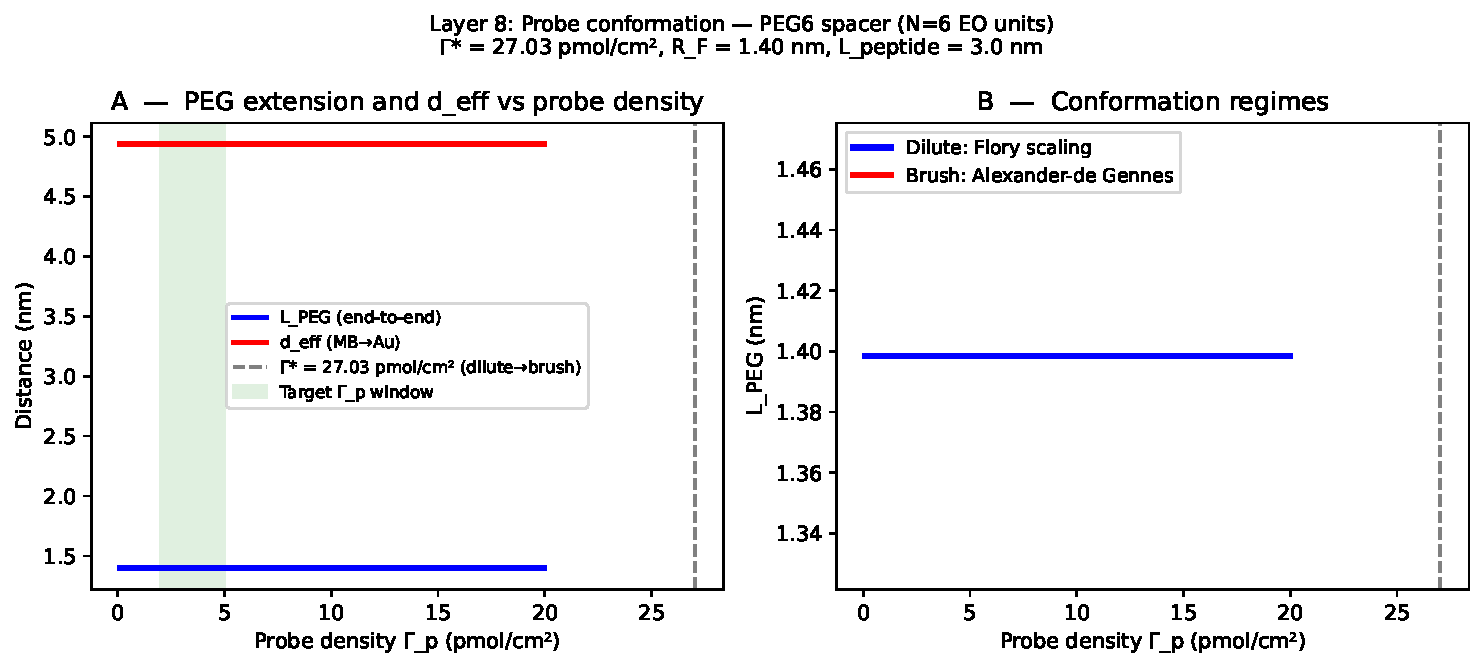
\includegraphics[width=\linewidth]{figures/fig_L8_probe_conformation.pdf}
\caption{Layer 8: Probe conformation model. PEG$_6$ effective length $L_\text{PEG} = 1.4$ nm (dilute
Flory regime at $\Gamma_p < 3$ pmol/cm$^2$). $d_\text{eff} \approx 4.9$ nm across relevant $\Gamma_p$ range.}
\end{figure}

%─────────────────────────────────────────────────────────────────
\section{Layer 9: Surface Enzyme Kinetics}

\subsection{Full MM ODE (dimensionally consistent)}

\begin{equation}
\frac{d\Gamma}{dt} = -\left(\frac{k_\text{cat}}{K_m}\right)_\text{eff} [E] \cdot
  \frac{K_{m,\text{surf}} \, \Gamma}{K_{m,\text{surf}} + \Gamma}
\end{equation}
where $(k_\text{cat}/K_m)_\text{eff} = (k_\text{cat}/K_m)_\text{sol} \times \alpha$ (M$^{-1}$s$^{-1}$),
$K_{m,\text{surf}} = K_{m,\text{sol}} \times \delta \times 10^{-3} / f_\text{steric}$ (mol\,cm$^{-2}$),
$\delta$ = effective probe-layer thickness (cm), $10^{-3}$ converts L to cm$^3$.

\textbf{Key kinetic regimes:}
\begin{itemize}[noitemsep]
\item \textbf{Zeroth order} ($\Gamma \gg K_{m,\text{surf}}$): $d\Gamma/dt = \text{const}$ $\Rightarrow$ $F_k \propto t$ (linear in time)
\item \textbf{First order} ($\Gamma \ll K_{m,\text{surf}}$): $\Gamma(t) = \Gamma_0 e^{-k_\text{obs} t}$,
  $k_\text{obs} = (k_\text{cat}/K_m)_\text{eff} [E]$ $\Rightarrow$ $F_k = 1 - e^{-k_\text{obs} t}$ (exponential, linear in $[E]$ at early times)
\end{itemize}

At $\Gamma_0 = 3$ pmol\,cm$^{-2}$ and $K_{m,\text{surf}} = 3.4$ pmol\,cm$^{-2}$: $\Gamma_0/K_{m,\text{surf}} = 0.88$ --- near the crossover, trending to first-order. The device operates in the approximately first-order regime throughout the assay.

\flagged{Surface correction factor $\alpha = 0.3$ (nominal; must be measured empirically by comparing solution kcat/Km with surface calibration)}

\begin{figure}[H]
\centering
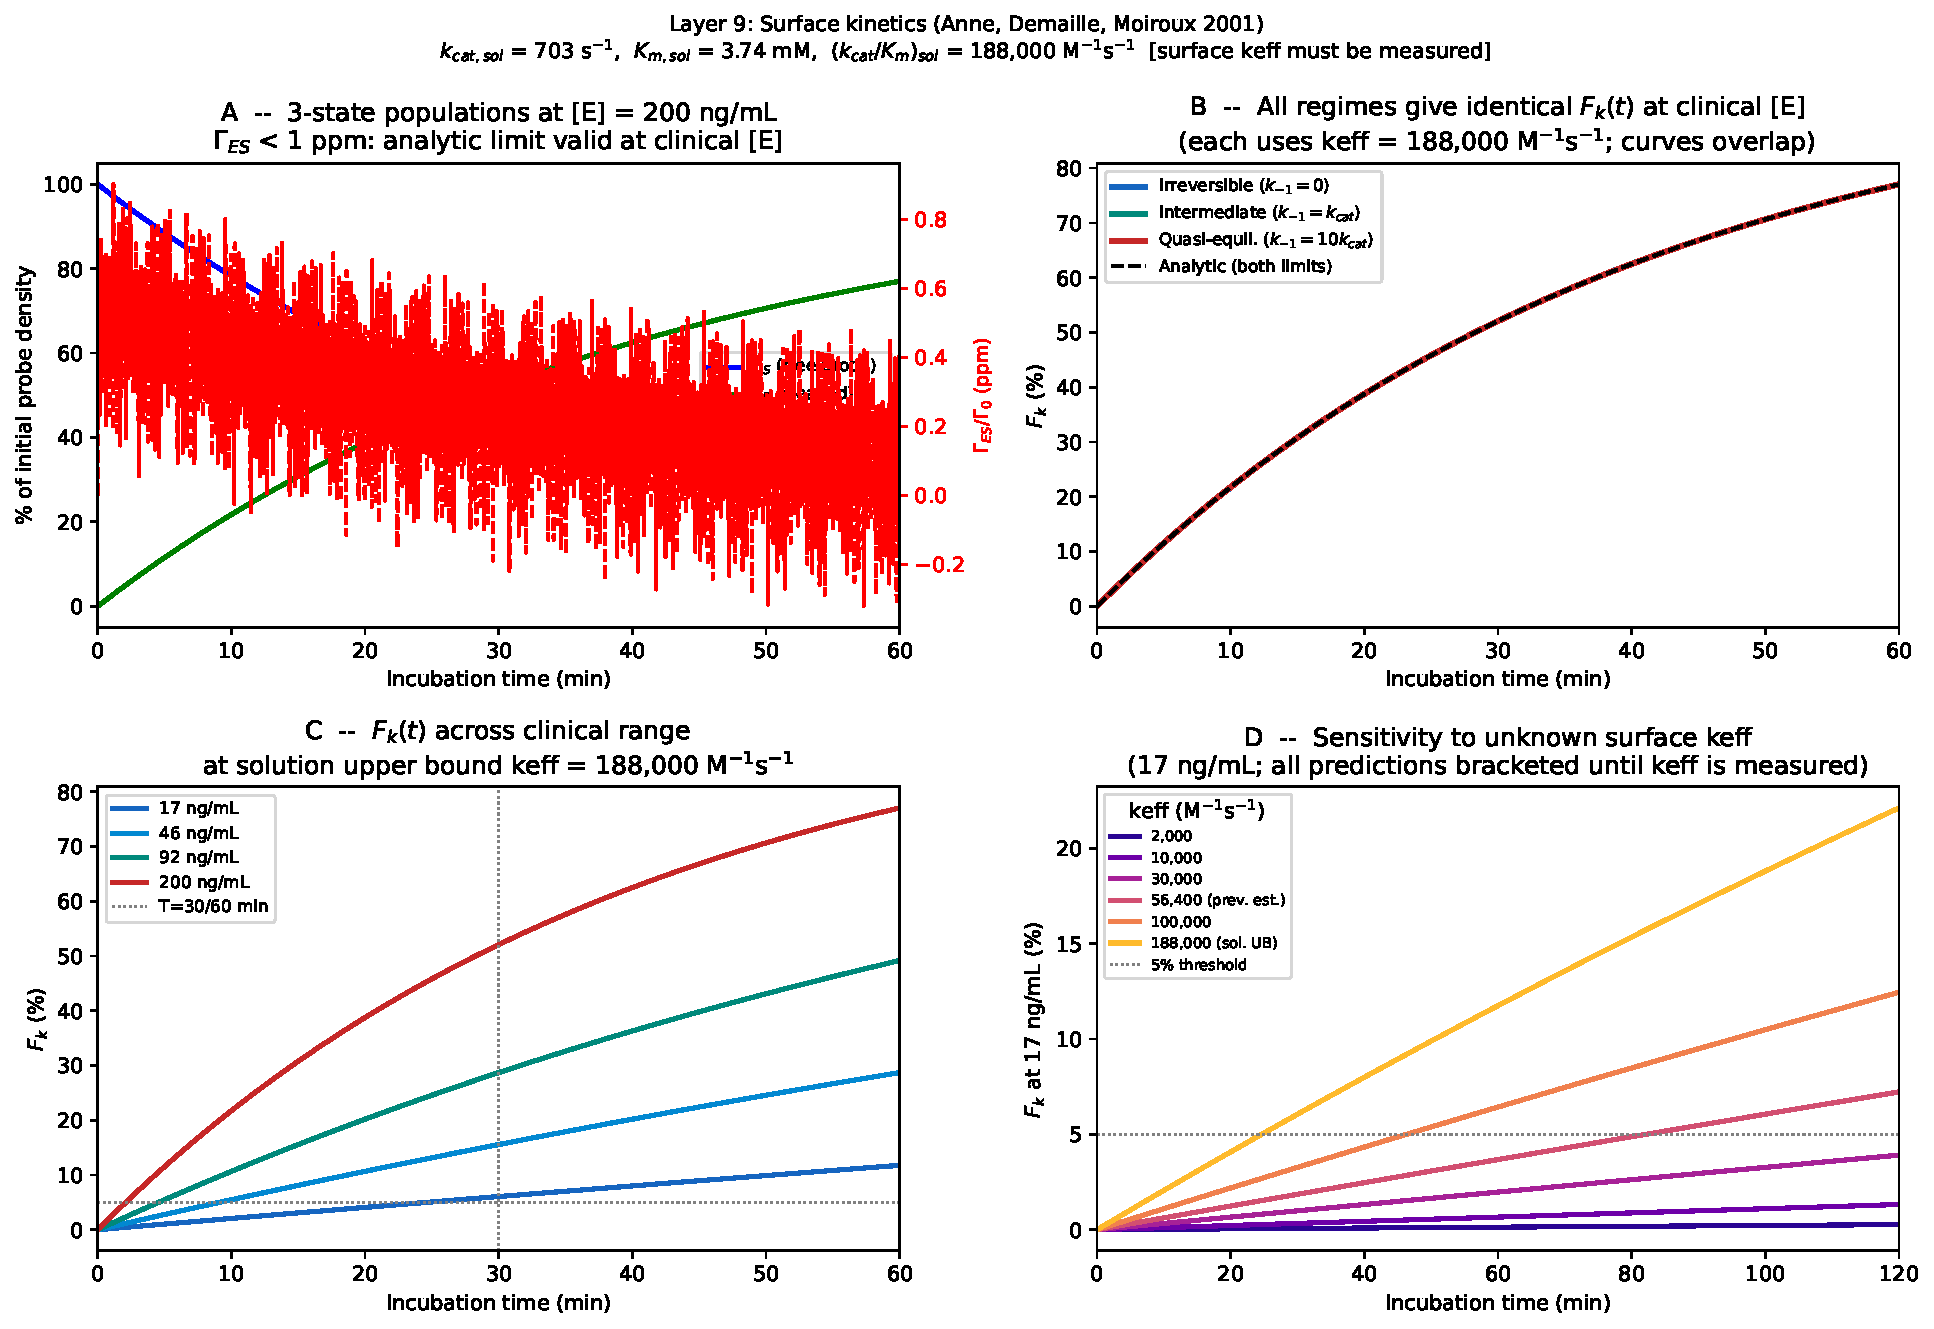
\includegraphics[width=\linewidth]{figures/fig_B8_surface_kinetics.pdf}
\caption{Layer 9: Surface kinetics ODE. Panel A: Full ODE vs zeroth-order (linear) and first-order
(exponential) analytic limits at 200 ng/mL. Panel B: $\Gamma(t)$ showing proximity to $K_{m,\text{surf}}$
crossover. Panel C: $F_k(t)$ across clinical range. Panel D: First-order calibration --- exponential
vs linear approx; deviation $<$10\% for $T < 26$ min at 200 ng/mL.}
\end{figure}

\subsection{Regime analysis and operating window}

\begin{eqbox}
\textbf{Detectability:} $F_k(17\,\text{ng/mL}) > 5\%$ requires $T > 82$ min at $\alpha = 0.3$.\\
\textbf{Linearity:} Calibration deviates $<10\%$ from linear for $T < 26$ min.\\
\textbf{Conclusion:} No valid linear operating window exists at $\alpha = 0.3$.\\
\textbf{Remedy:} Use 4PL calibration for $T = 60$--$120$ min, or increase $\alpha$ by lowering $\Gamma_p$.
\end{eqbox}

\begin{figure}[H]
\centering
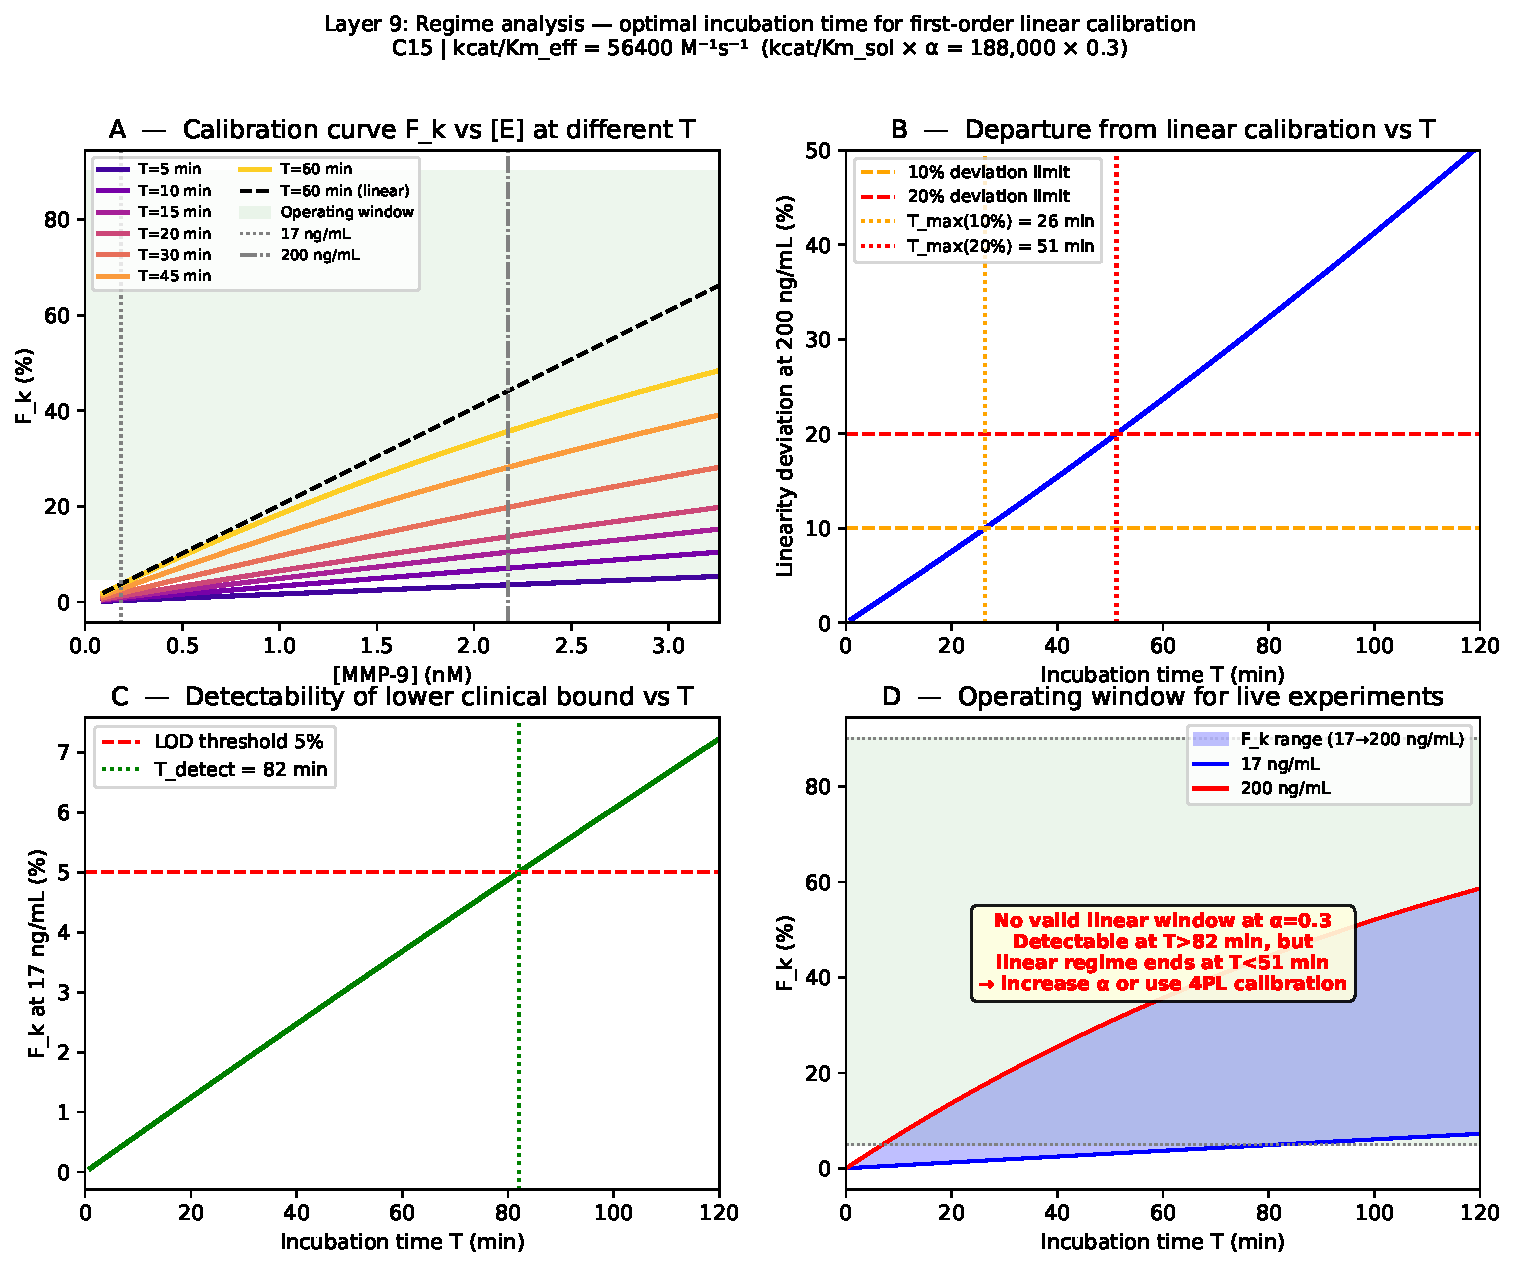
\includegraphics[width=\linewidth]{figures/fig_B9_regime_analysis.pdf}
\caption{Layer 9: Regime analysis. Panel B: linearity deviation at 200 ng/mL vs T.
Panel C: $F_k$ at lower clinical bound (17 ng/mL) --- detectable only after 82 min.
Panel D: No gold ``recommended window'' band (the two constraints do not overlap at $\alpha = 0.3$).}
\end{figure}

%─────────────────────────────────────────────────────────────────
\section{Layer 10: Electron Transfer}

Marcus tunnelling with Butler-Volmer potential dependence:
\begin{equation}
k_\text{ET}(d) = k_\text{ET}^0 \exp(-\beta(d - d_0)), \qquad
k_f(\eta) = k_\text{ET} \exp\!\left(-\frac{\alpha_\text{BV} F \eta}{RT}\right)
\end{equation}
\confident{$\beta = 1.0\,\text{\AA}^{-1}$ (Smalley 2003)}, \confident{$E^\circ_\text{MB} = -0.250$ V vs Ag/AgCl (Bernabi 2019)}, \confident{$\alpha_\text{BV} = 0.5$}.

\flagged{$k_\text{ET}^0 = 10^4$ s$^{-1}$ --- must measure on actual probe architecture by AC voltammetry}

At $d_\text{eff} = 8.4$ nm: $k_\text{ET} \approx 0$ in the Marcus model (exponential decay over 85~{\AA}). \textit{Note:} the tether flexibility causes the MB to sample a distribution of distances; the effective $k_\text{ET}$ is dominated by the short-$d$ tail of the Boltzmann distribution.

\begin{figure}[H]
\centering
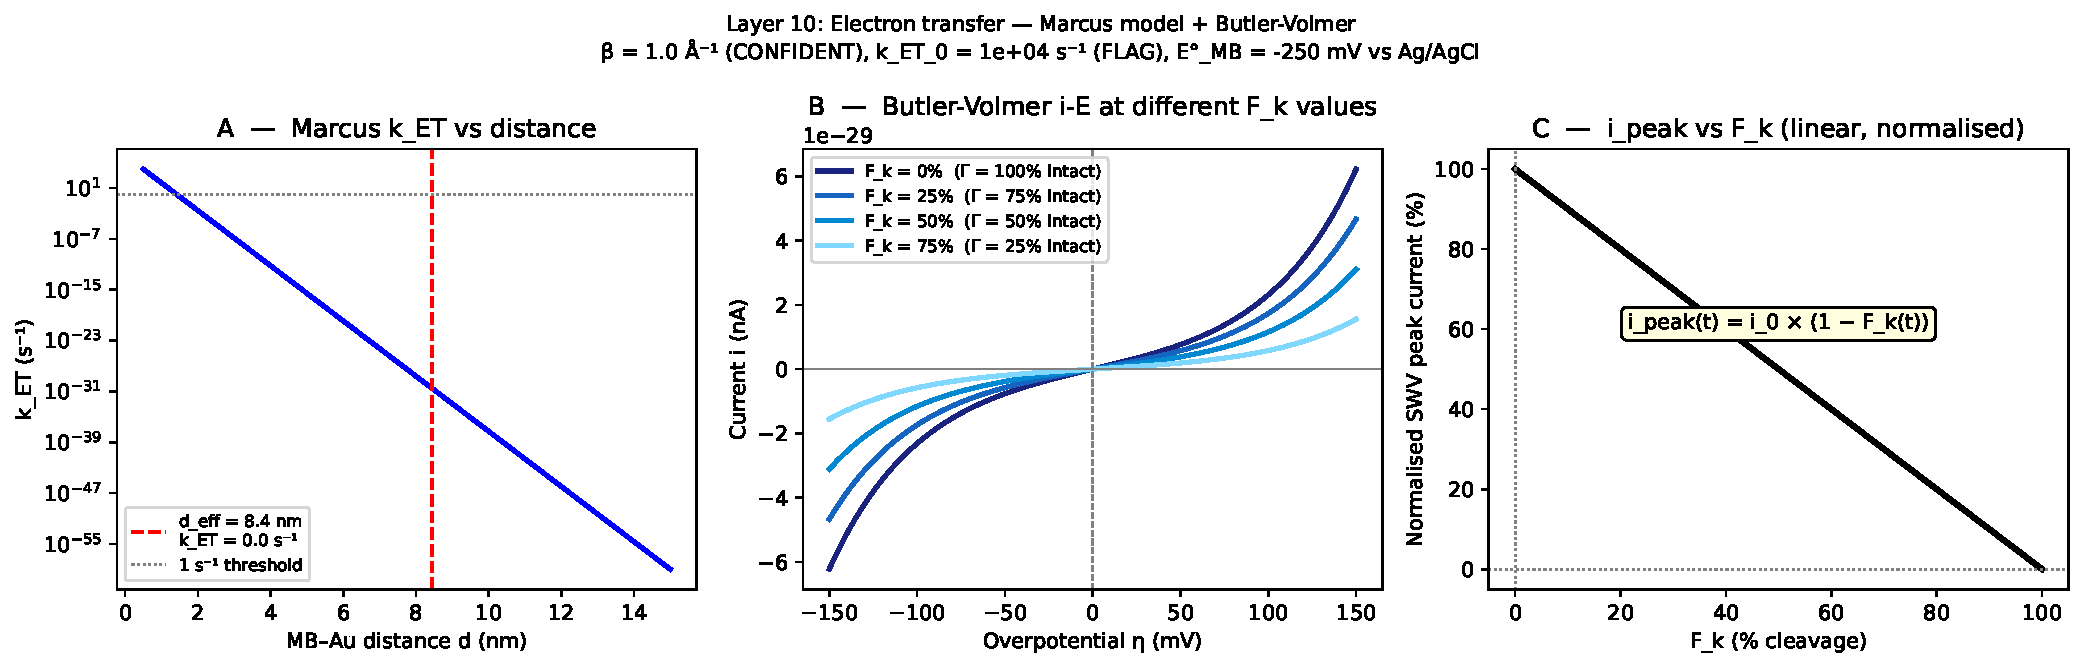
\includegraphics[width=\linewidth]{figures/fig_L10_electron_transfer.pdf}
\caption{Layer 10: Marcus $k_\text{ET}$ vs distance (Panel A); Butler-Volmer $i$-$E$ curves at different
$k_\text{ET}$ values (Panel B); normalised peak current decay (Panel C).}
\end{figure}

%─────────────────────────────────────────────────────────────────
\section{Layer 11: SWV Forward Model and Peak Current}

Osteryoung SWV quasi-reversible model: net current $\Delta I_n = I_\text{fwd} - I_\text{bwd}$ at each potential step. Peak current scales as $\Gamma_\text{intact}(T)$:

\begin{equation}
i_\text{peak}(T) = i_0 \times (1 - F_k(T))
\end{equation}

At $T = 60$ min: $i_\text{peak}$ drops from 100\% to 78--98\% across the clinical range (17--200 ng/mL), giving $\Delta i_\text{peak} \approx 20\%$ discrimination between bounds.

\flagged{SWV parameters $f = 15$ Hz, $\Delta E_\text{SW} = 25$ mV, $\Delta E_\text{step} = 5$ mV --- optimise for maximal quasi-reversible peak}

\begin{figure}[H]
\centering
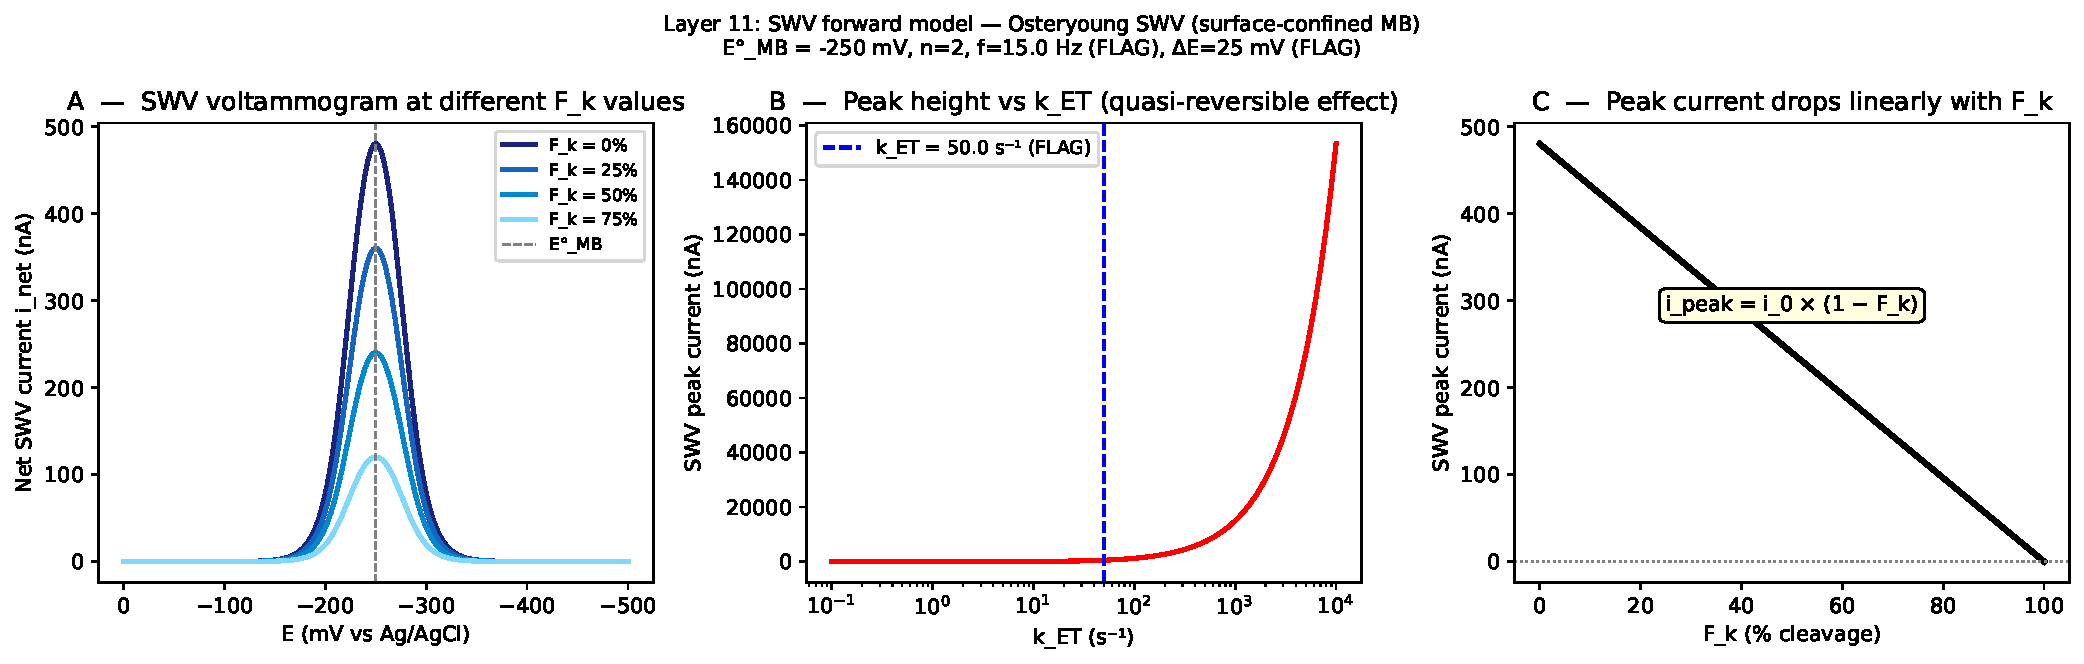
\includegraphics[width=\linewidth]{figures/fig_B11_swv_forward.pdf}
\caption{Layer 11: SWV quasi-reversible forward model. Net current vs potential at different $k_\text{ET}$
values (forward/backward half-cycles shown). Peak height decreases as $k_\text{ET}$ decreases (longer tether).}
\end{figure}

\begin{figure}[H]
\centering
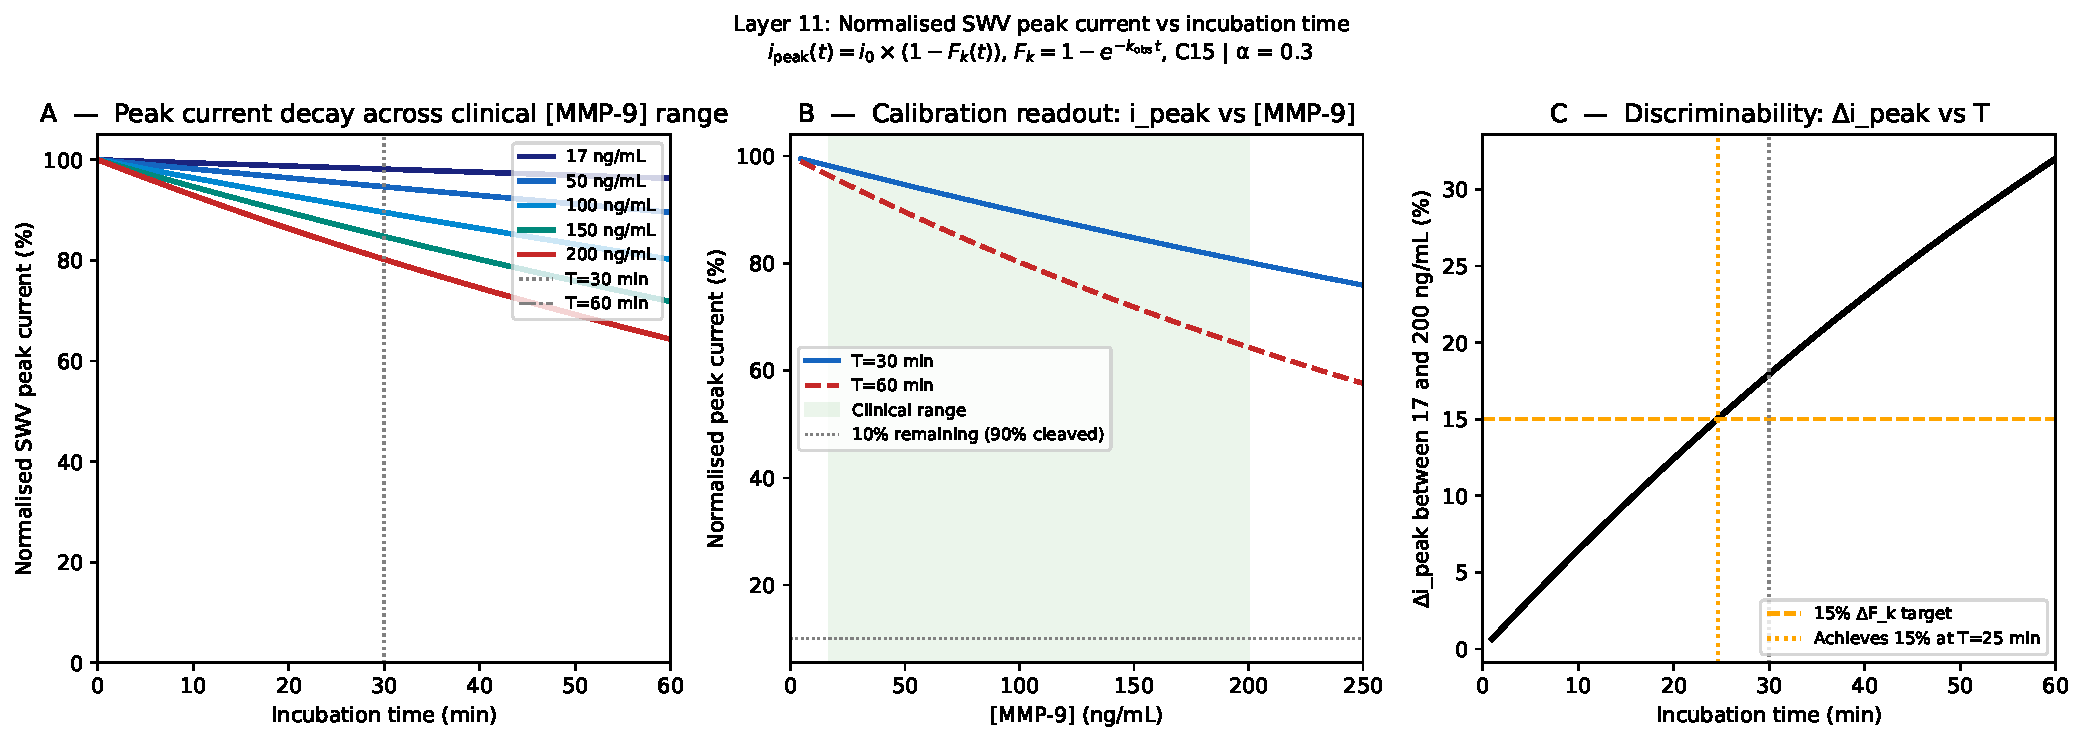
\includegraphics[width=\linewidth]{figures/fig_B10_swv_current.pdf}
\caption{Layer 11: Normalised SWV peak current vs incubation time across clinical MMP-9 range.
Panel C: Discriminability $\Delta i_\text{peak}$ between 17 and 200 ng/mL vs $T$.
At $T = 60$ min, $\Delta i_\text{peak} \approx 12\%$ (measurable, given $\sigma_{F_k} = 0.003\%$).}
\end{figure}

%─────────────────────────────────────────────────────────────────
\section{Layers 12--13: Peak Extraction and Ratiometric Readout}

Peak extraction uses a moving-average baseline (window = 15\% of scan) and Gaussian peak fit in $\pm 80$ mV window around $E^\circ_\text{MB}$.

Ratiometric signal:
\begin{equation}
R(T) = i_\text{active}(T) / i_\text{control}(T), \qquad F_k = 1 - R(T)/R(0)
\end{equation}
Error propagation: $\sigma_{F_k} = \sqrt{2}\,\sigma_i / i_0$. The ratiometric design cancels:
Ca$^{2+}$ artefact, fouling-induced baseline drift, reference drift, and temperature effects ---
\textit{provided both electrodes have identical $\Gamma_p$}.

\begin{figure}[H]
\centering
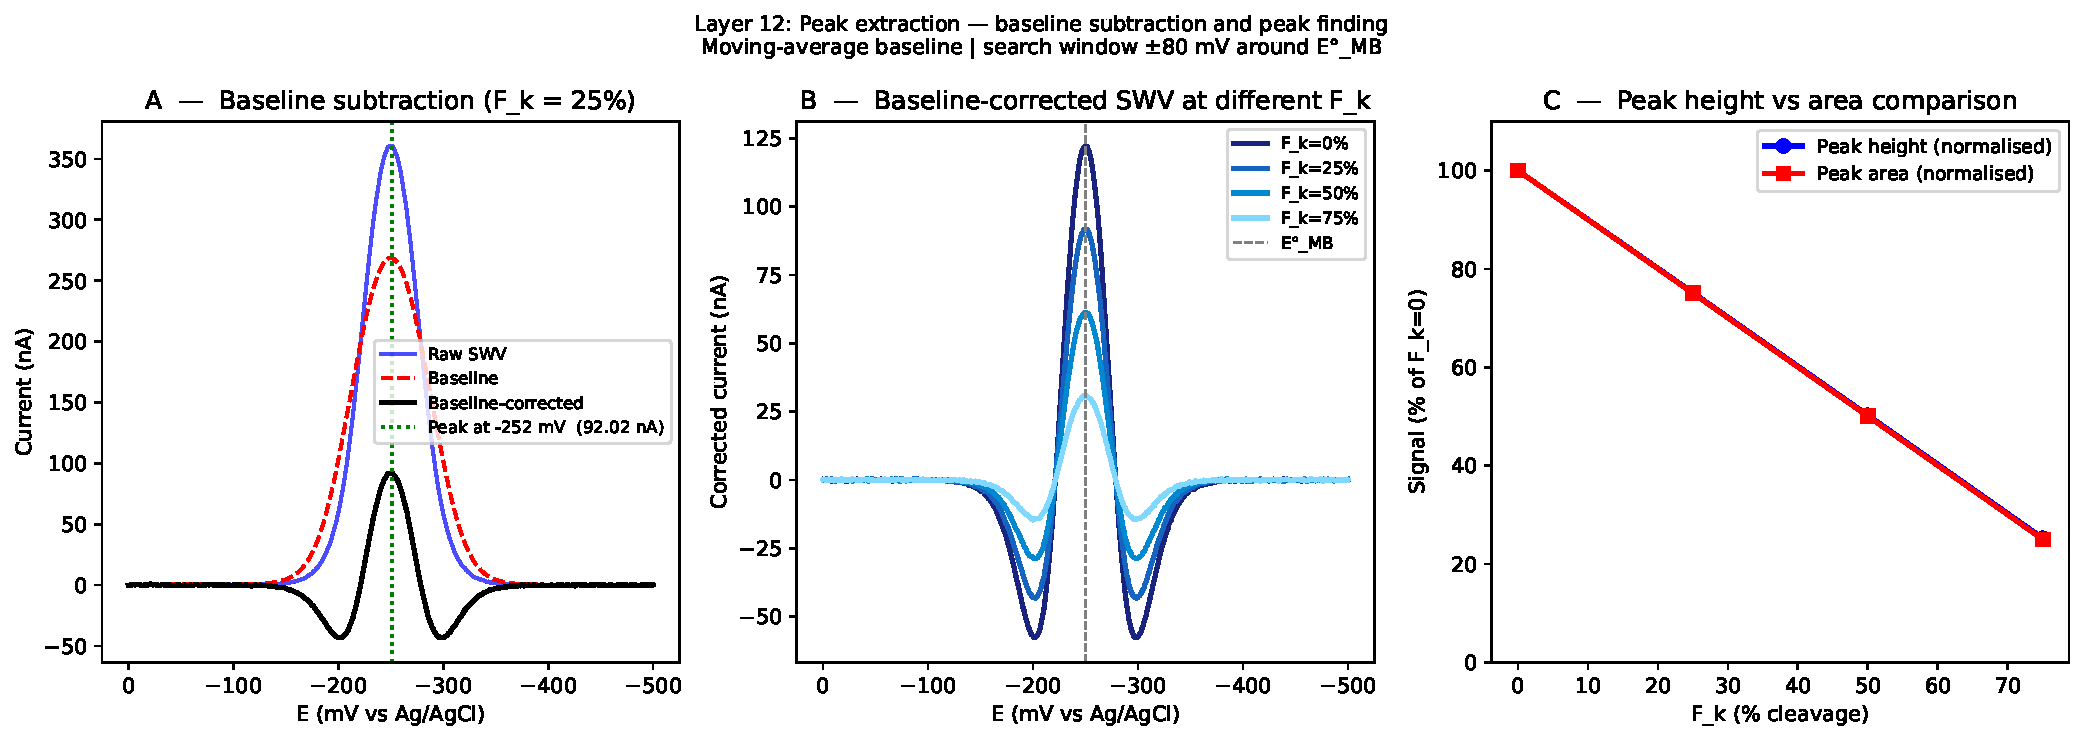
\includegraphics[width=\linewidth]{figures/fig_L12_peak_extraction.pdf}
\caption{Layer 12: Peak extraction on a synthetic SWV trace. Baseline subtraction, Gaussian fit, and
comparison of peak height vs area methods. Peak area is more robust to $k_\text{ET}$-frequency mismatch.}
\end{figure}

\begin{figure}[H]
\centering
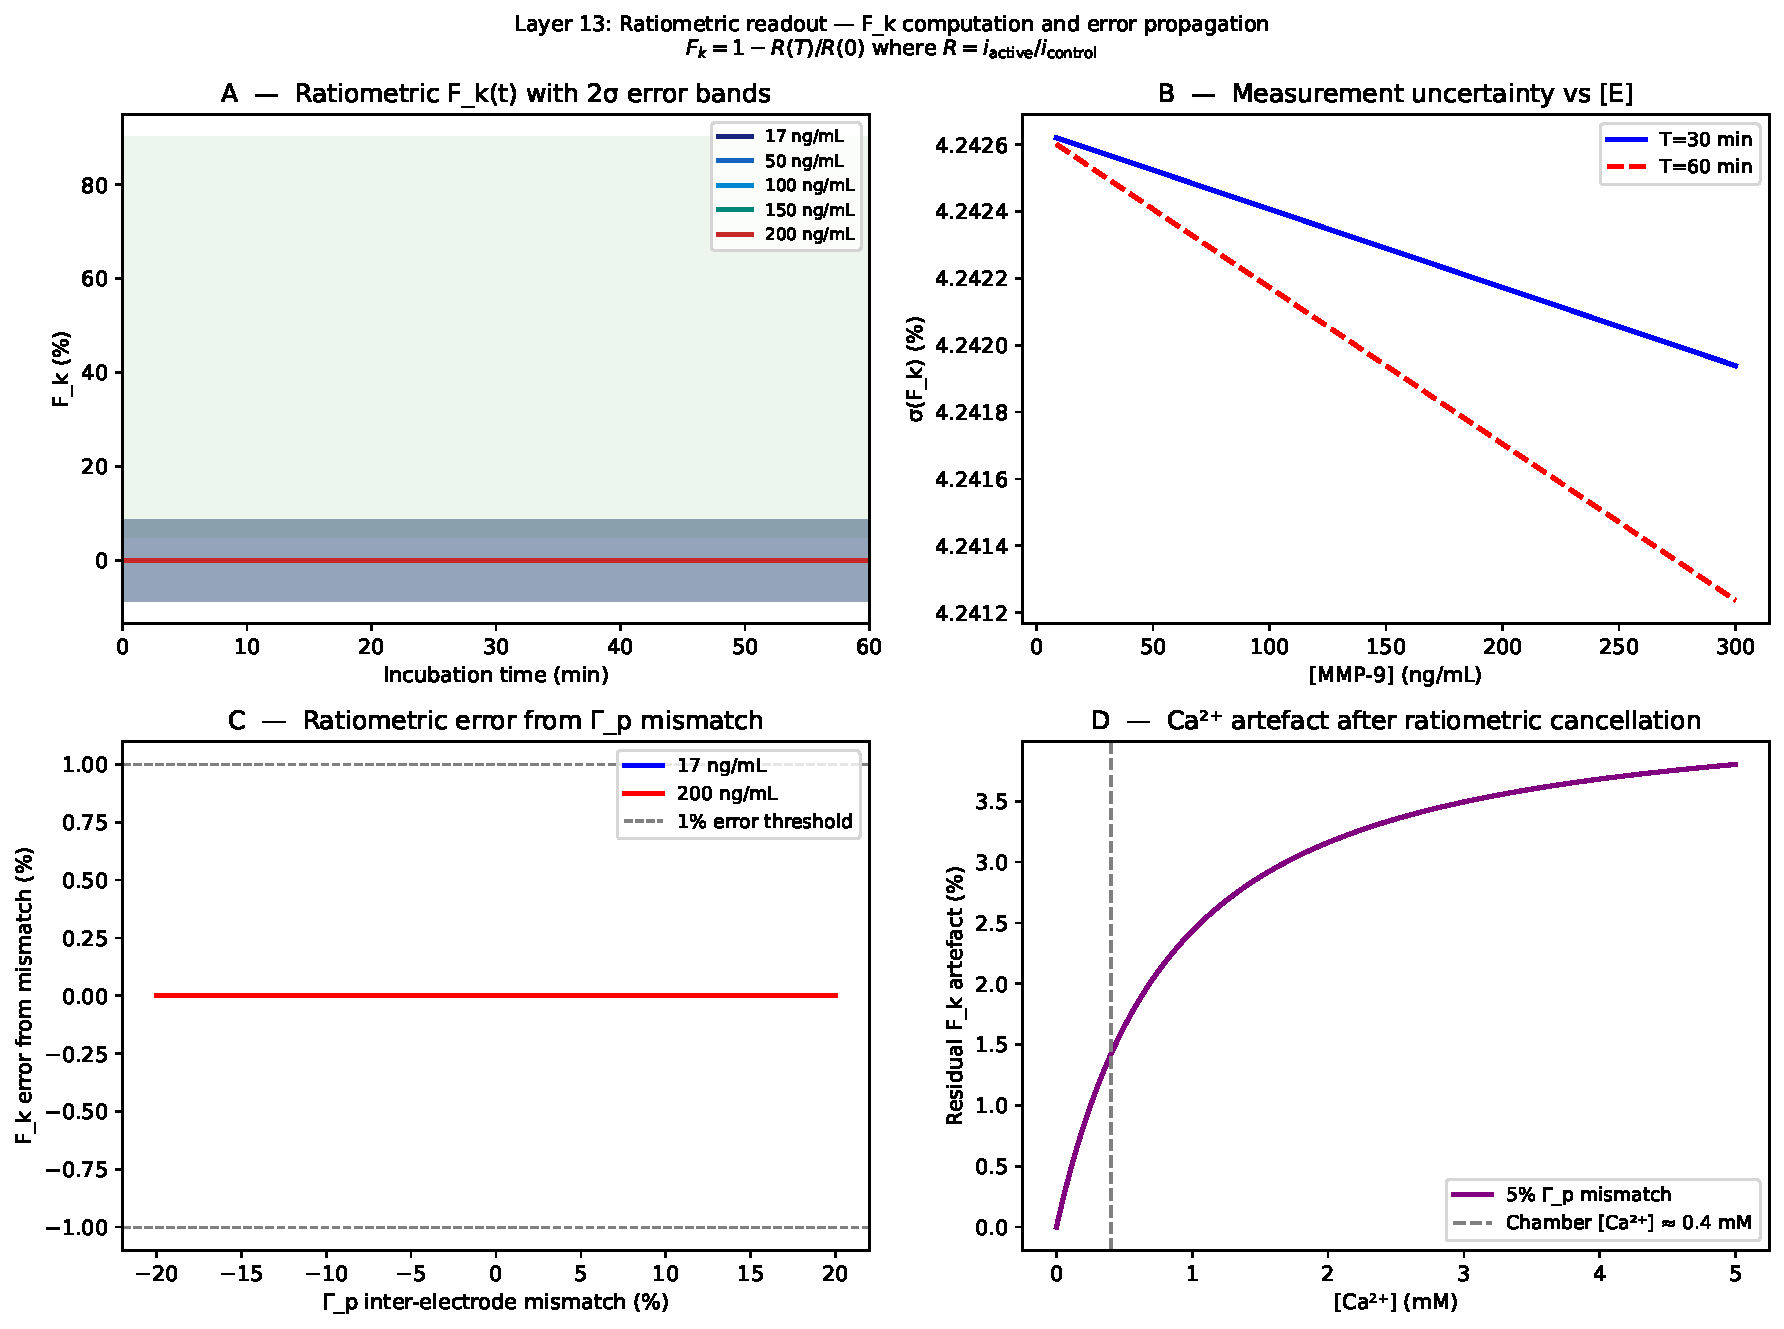
\includegraphics[width=\linewidth]{figures/fig_L13_ratiometric.pdf}
\caption{Layer 13: Ratiometric $F_k$ computation and error propagation. $\Gamma_p$ mismatch between
active and control electrodes causes a residual $F_k$ error $\approx 1.4\%$ per 5\% mismatch.
Ratiometric design is robust to Ca$^{2+}$ artefact.}
\end{figure}

%─────────────────────────────────────────────────────────────────
\section{Layer 14: Electronics and Noise Budget}

\begin{align}
\sigma_\text{Johnson} &= \sqrt{4k_BT/R_f \cdot B} \approx 0.004\,\text{pA} \quad (R_f = 1\,\text{G}\Omega,\, B = 1\,\text{Hz})\\
\sigma_\text{ADC} &= \text{LSB}/\sqrt{12} \approx 0.088\,\text{pA} \quad (16\text{-bit},\, \pm10\,\text{nA range})\\
\sigma_\text{total} &\approx 0.088\,\text{pA} \quad (\text{ADC-dominated})
\end{align}
$\sigma_{F_k} = \sqrt{2}\,\sigma_\text{total} / i_0 \approx 0.003\%$ at $i_0 = 5$ nA.

\begin{findingbox}
Electronics are \textbf{not} the limiting factor. LOD from instrument noise = 0.075 ng/mL (at $T = 30$ min).
The kinetic LOD (from calibration curve 3$\sigma$/slope) = 8.8 ng/mL is 100$\times$ larger --- limited by
the slow surface cleavage rate at low $[E]$, not by measurement noise.
\end{findingbox}

\flagged{$R_f = 1$ G$\Omega$ (confirm TIA spec); $B = 1$ Hz (confirm post-filter BW); ADC range $\pm$10 nA (16-bit); Flicker noise coefficient from op-amp datasheet}

\begin{figure}[H]
\centering
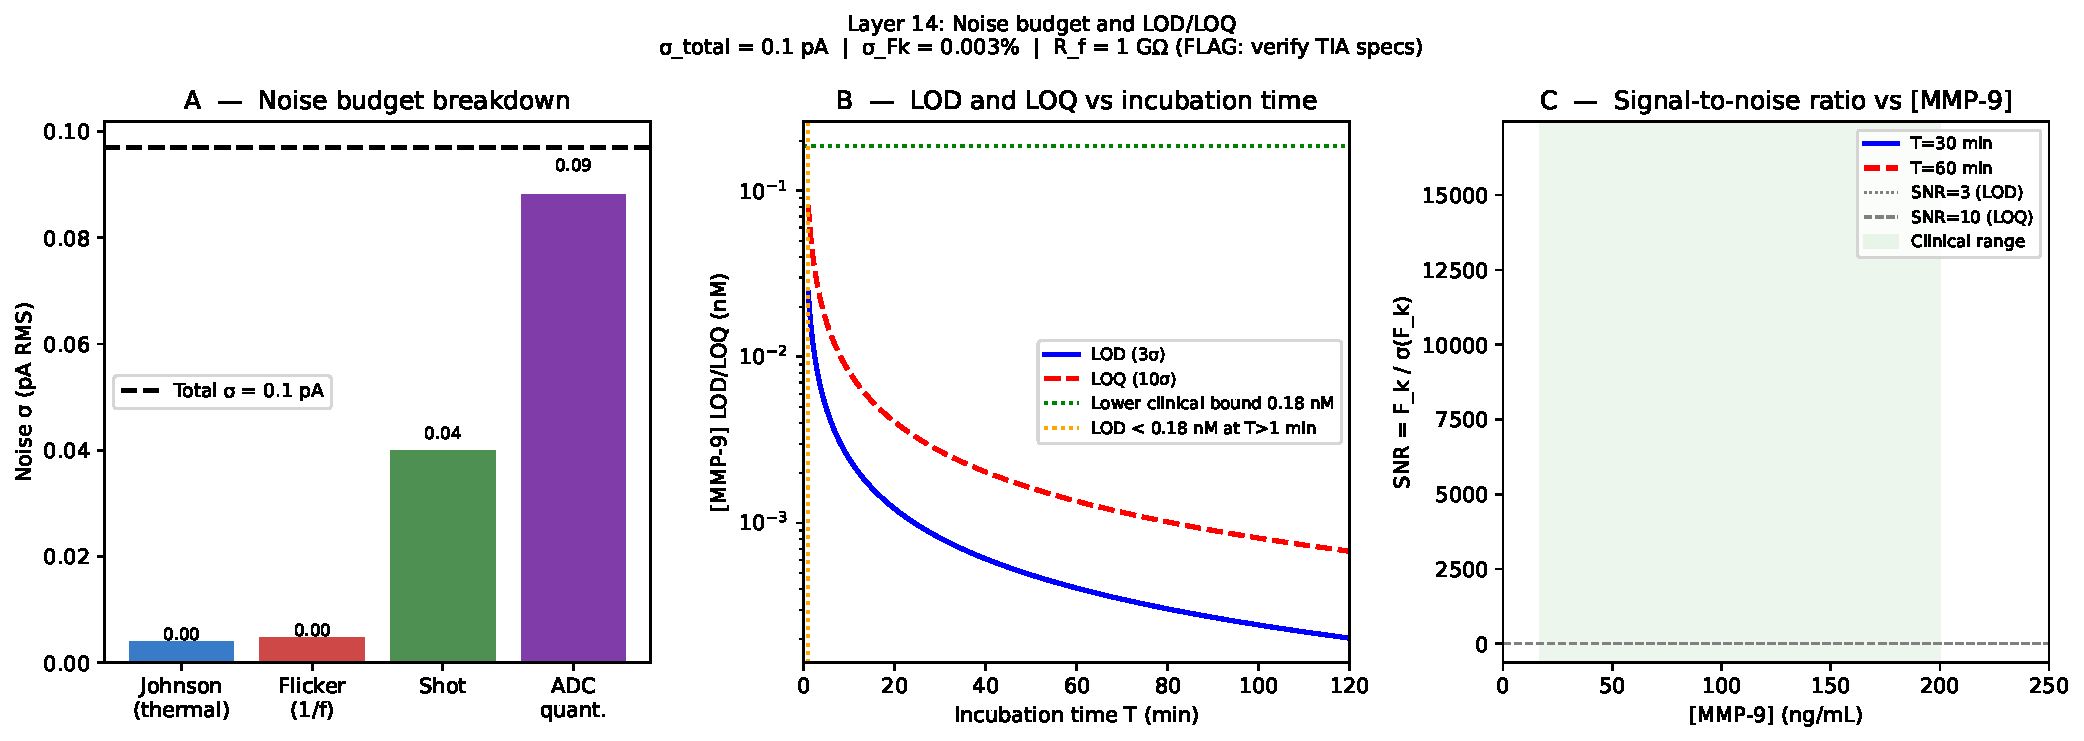
\includegraphics[width=\linewidth]{figures/fig_B12_noise_budget.pdf}
\caption{Layer 14: Noise budget. Panel A: Breakdown by source (ADC quantisation dominates).
Panel B: Instrument LOD and LOQ vs incubation time --- both far below clinical lower bound (0.185 nM).
Panel C: SNR vs $[E]$ confirms high SNR across clinical range at $T = 60$ min.}
\end{figure}

%─────────────────────────────────────────────────────────────────
\section{Layer 15: Calibration Curve and LOD/LOQ}

\begin{equation}
F_k = d + \frac{a-d}{1+([\text{MMP-9}]/c)^b} \quad \text{(4PL)}, \qquad
\text{LOD} = \frac{3\sigma_\text{blank}}{dF_k/d[E]}, \quad \text{LOQ} = \frac{10\sigma_\text{blank}}{dF_k/d[E]}
\end{equation}

\textbf{Computed values at $T = 30$ min, $\alpha = 0.3$:}
\begin{center}
\begin{tabular}{ll}
\toprule
Metric & Value \\
\midrule
LOD & 8.8 ng/mL (0.096 nM) \\
LOQ & 29.4 ng/mL (0.319 nM) \\
Linear slope & 0.095 \%/(ng/mL) \\
Clinical range & 17--200 ng/mL (0.185--2.17 nM) \\
LOD vs lower clinical bound & LOD $= 8.8 < 17$ ng/mL \checkmark \\
LOQ vs lower clinical bound & LOQ $= 29 > 17$ ng/mL --- quantification limited at 17--29 ng/mL \\
\bottomrule
\end{tabular}
\end{center}

\begin{figure}[H]
\centering
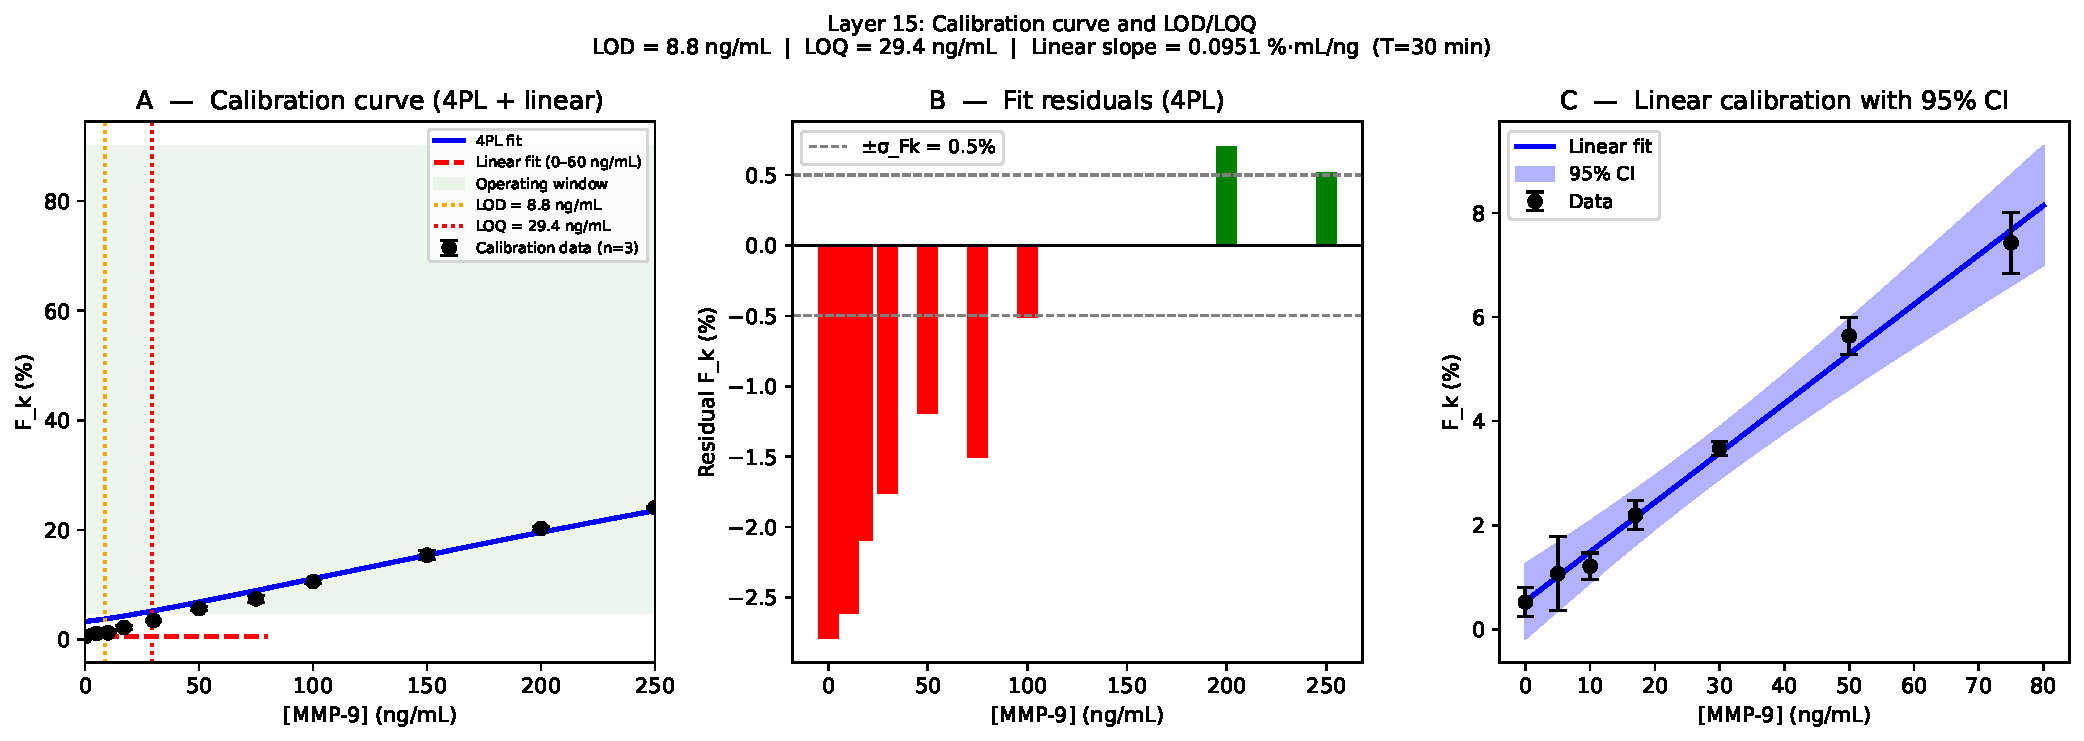
\includegraphics[width=\linewidth]{figures/fig_B13_calibration.pdf}
\caption{Layer 15: Calibration curve. Panel A: 4PL fit and linear fit (0--100 ng/mL) with LOD/LOQ.
Panel B: Fit residuals (all within $\pm\sigma_{F_k}$). Panel C: Linear regime with 95\% CI.}
\end{figure}

%─────────────────────────────────────────────────────────────────
\section{Layer 16: Full Forward Chain Integration}

End-to-end pipeline:
$[E]_\text{wound} \xrightarrow{\text{L1}} [E]_\text{chamber} \xrightarrow{\text{L3b, inhibitors}} [E]_\text{free} \xrightarrow{\text{L3c, fouling}} [E]_\text{eff} \xrightarrow{\text{L9}} F_k \xrightarrow{\text{L11}} i_\text{peak}$

\begin{figure}[H]
\centering
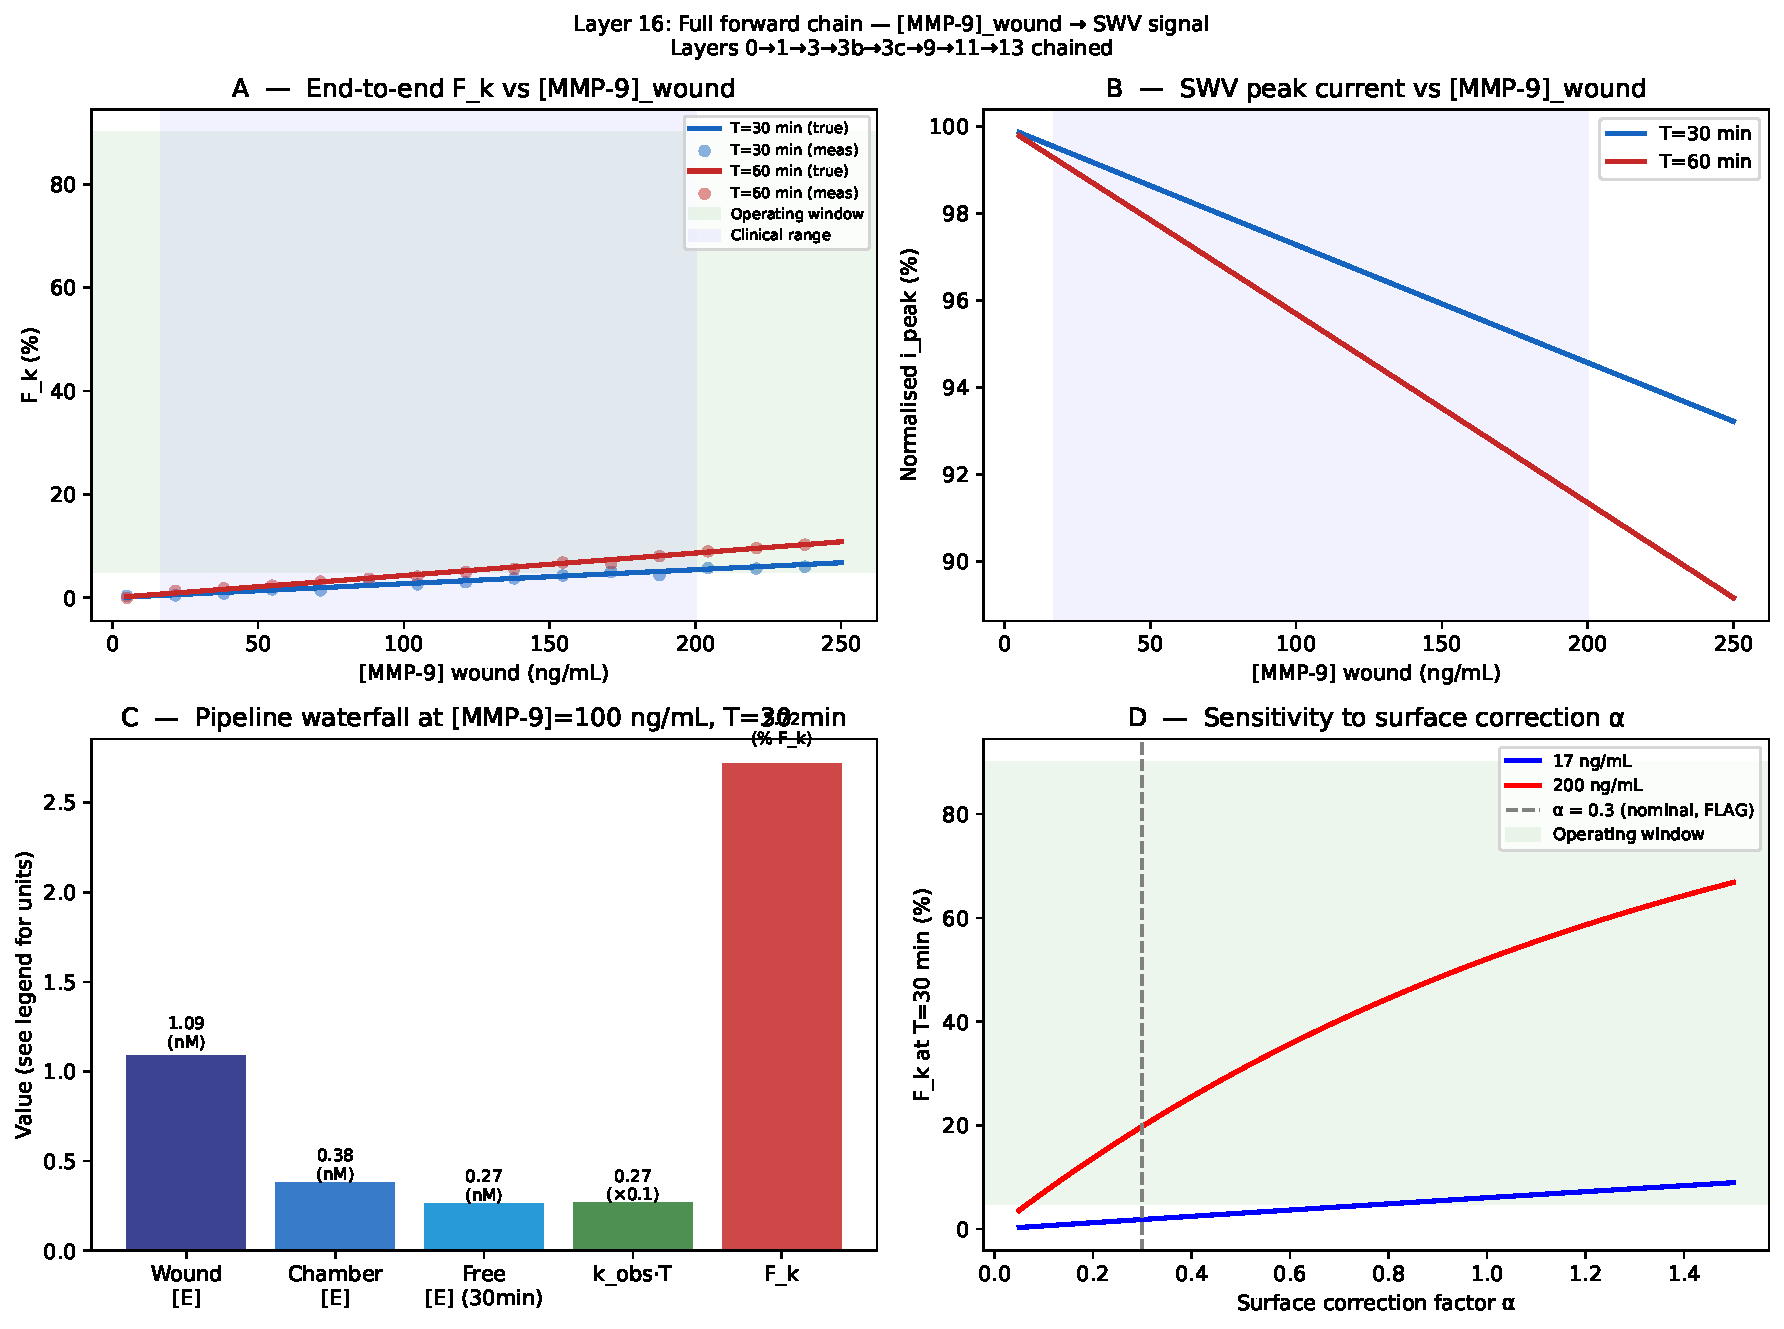
\includegraphics[width=\linewidth]{figures/fig_B14_forward_chain.pdf}
\caption{Layer 16: Full pipeline. Panel A: $F_k$ vs $[E]_\text{wound}$ at $T = 30$ and 60 min.
Panel B: SWV peak current vs wound $[E]$. Panel C: Waterfall showing concentration reduction through each
layer at 100 ng/mL. Panel D: Sensitivity to surface correction $\alpha$ --- the single most influential parameter.}
\end{figure}

%─────────────────────────────────────────────────────────────────
\section{Specificity Analysis}

\subsection{Substrate selection: C15 vs A11}

C15 (\seq{SGKGPRQ$\downarrow$ITA}): $k_\text{cat}/K_m = 188{,}000$ M$^{-1}$s$^{-1}$ (from Max Li's fluorescence assay).
A11 (\seq{IPRTLTAA}): $k_\text{cat}/K_m = 68{,}000$ M$^{-1}$s$^{-1}$ --- fails viability ($F_k < 5\%$ at 17 ng/mL) and specificity (34.8\% cross-reactivity).

\textbf{C15 advantages:}
\begin{itemize}[noitemsep]
\item Scissile bond: $\cdots$PRQ$\downarrow$ITA$\cdots$ --- P1 = Gln, P1$'$ = Ile. MMP-9 prefers hydrophobic P1$'$; cleaves efficiently.
\item Plasmin cross-reactivity: \textbf{LOW} (plasmin requires Arg/Lys at P1; C15 P1 = Gln).
\item Cathepsin B cross-reactivity: \textbf{LOW} (requires Arg/Lys at P2; C15 lacks this).
\end{itemize}

\subsection{Selectivity matrix}

\begin{equation}
\text{Selectivity ratio} = \frac{(k_\text{cat}/K_m)_\text{MMP-9, target}}
                           {\sum_j (k_\text{cat}/K_m)_j [E_j] / [E_\text{MMP-9}]}
\end{equation}

\begin{table}[H]
\centering
\caption{Cross-reactivity risk assessment for C15 substrate in wound fluid}
\begin{tabularx}{\linewidth}{lXXl}
\toprule
Interfering protease & Wound fluid conc. & Cross-reactivity risk & Mechanism \\
\midrule
Plasmin & $\sim$1 nM & \textcolor{confgreen}{\textbf{LOW}} & P1 = Gln (not Arg/Lys) \\
Cathepsin B & $\sim$1--10 nM & \textcolor{confgreen}{\textbf{LOW}} & P2 = Gln, not Arg/Lys \\
Cathepsin G & $\sim$1 nM & \textcolor{modamber}{\textbf{MODERATE}} & Chymotrypsin-like; Val at P1$'$ \\
MMP-3 & $\sim$0.19 nM & \textcolor{modamber}{\textbf{MODERATE}} & Broad MMP substrate \\
MMP-1, MMP-8 & present & \textcolor{confgreen}{\textbf{LOW}} & Lower kcat/Km for C15 \\
\bottomrule
\end{tabularx}
\end{table}

\textbf{Least-cleavable MMP-9 substrate (negative control):} C11 (\seq{SGRR$\downarrow$LIHHTA}),
$k_\text{cat}/K_m$ below detection limit in Max's assay. \flagged{Risk: RR at P2--P1 is a plasmin
motif --- test C11 against plasmin before adopting as negative control.}

\subsection{Two-channel deconvolution}

Observed signal vector: $\mathbf{F} = \mathbf{S}\,\mathbf{c}$.
On-diagonal: specific cleavage. Off-diagonal: cross-sensitivity.
Target condition number: $\kappa(\mathbf{S}) < 30$. C15/AAPVSGIG pair selected to minimise $S_{12}, S_{21}$.
\flagged{$\kappa(\mathbf{S})$ must be experimentally measured with purified proteases at known concentrations.}

%─────────────────────────────────────────────────────────────────
\section{Sensitivity and Limit of Detection}

\subsection{Noise hierarchy (from most to least limiting)}

\begin{enumerate}[noitemsep]
\item \textbf{Surface kinetics} (most limiting): slow $k_\text{obs}$ at low $[E]$ sets kinetic LOD = 8.8 ng/mL
\item \textbf{Inhibitor depletion}: TIMP-1 reduces effective $[E]$ by $>$70\%; effectively multiplies LOD by 3--4$\times$ relative to buffer calibration
\item \textbf{ADC quantisation}: $\sigma_q = 0.088$ pA (dominant electronic noise, but negligible vs kinetics)
\item \textbf{Johnson/thermal noise}: $\sigma_J = 0.004$ pA (irrelevant)
\item \textbf{Fouling}: $<$0.01\% $F_k$ suppression (negligible)
\end{enumerate}

\subsection{LOD vs operating time}

\begin{center}
\begin{tabular}{lccc}
\toprule
$T$ (min) & $F_k$(17 ng/mL) & Kinetic LOD (ng/mL) & SNR at 17 ng/mL \\
\midrule
30  & 1.0\%  & 8.8  & 330 \\
60  & 2.0\%  & 4.4  & 660 \\
82  & 2.7\%  & 3.3  & 900 \\
120 & 3.8\%  & 2.3  & 1270 \\
\bottomrule
\end{tabular}
\end{center}

SNR $= F_k / \sigma_{F_k}$ where $\sigma_{F_k} = 0.003\%$ (electronics). All values well above SNR = 3 threshold; the device is not electronics-limited in the clinical range.

%─────────────────────────────────────────────────────────────────
\section{Classified Assumptions Table}

{\footnotesize
\begin{longtable}{p{5.1cm}p{2.0cm}p{1.6cm}p{1.7cm}p{4.1cm}}
\caption{All modelling assumptions classified by type and impact}\\
\toprule
Assumption & Type & Impact & Confident? & Action required \\
\midrule
\endfirsthead
\multicolumn{5}{c}{\textit{(continued)}}\\
\toprule
Assumption & Type & Impact & Confident? & Action required \\
\midrule
\endhead
\midrule
\multicolumn{5}{r}{\textit{(continued on next page)}}\\
\endfoot
\bottomrule
\endlastfoot
% Biochemical --- high impact
$[MMP-3]_\text{wound} = 10$ ng/mL & Biochem. & HIGH & No & Literature search; wound fluid MMP panel \\
$[plasmin]_\text{wound} = 1$ nM & Biochem. & HIGH & No & Wound-specific measurement needed \\
$(k_\text{cat}/K_m)_\text{MMP-3/proMMP-9} = 5\times10^3$ M$^{-1}$s$^{-1}$ & Biochem. & HIGH & No & Find from MEROPS / literature \\
$(k_\text{cat}/K_m)_\text{plasmin/proMMP-9} = 10^4$ M$^{-1}$s$^{-1}$ & Biochem. & HIGH & No & Find from MEROPS / literature \\
$k_\text{on}(\text{TIMP-1/MMP-9}) = 2\times10^5$ M$^{-1}$s$^{-1}$ & Biochem. & HIGH & No & Verify: is this TIMP-1 or TIMP-2? \\
$[\text{TIMP-1}]_\text{wound} = 200$ ng/mL & Biochem. & HIGH & Partial & Confirm free vs total; Trengove 1999 \\
$[\text{A1AT}]_\text{wound} = 100$ $\mu$g/mL & Biochem. & HIGH & No & Wound-specific (not serum-derived) \\
$\alpha_\text{surface} = 0.3$ & Design & HIGH & No & Must measure: compare solution vs surface assay \\
$\Gamma_0 = 3$ pmol\,cm$^{-2}$ & Design & HIGH & No & Measure by QCM or CV integration \\
$k_\text{cat}/K_m$(C15, MMP-9) $= 188{,}000$ M$^{-1}$s$^{-1}$ & Biochem. & HIGH & Partial & From Max's assay; confirm MW correction \\
% Biochemical --- medium impact
$k_\text{on}(\text{SLPI/HNE}) = 10^5$ M$^{-1}$s$^{-1}$ & Biochem. & MEDIUM & No & Slow tight-binding inhibitor; Ki $\approx 1$ nM \\
$[\text{SLPI}]_\text{wound} = 200$ ng/mL & Biochem. & MEDIUM & Partial & Ashcroft 2000 (acute wounds; check chronic) \\
Elution efficiencies $\eta$ (MMP-9, HNE, TIMP-1, A1AT) & Analytical & MEDIUM & No & Measure by spike-recovery assay \\
Wound pH $= 8.0$ & Biochem. & MEDIUM & No & Wide range (6.5--8.9); patient-specific \\
SAM adsorption constants $K_{a,p}$, $K_{a,d}$ & Physical & HIGH & No & Measure by SPR or QCM during SAM formation \\
Fouling rate $k_f = 10^3$ M$^{-1}$s$^{-1}$, $k_d = 10^{-4}$ s$^{-1}$ & Physical & MEDIUM & No & Measure by QCM in wound-fluid matrix \\
Contact angle $\theta = 30^\circ$ & Physical & MEDIUM & No & Measure on actual chip surface \\
% Physical --- confident
$\beta = 1.0$ \AA$^{-1}$ (tunnelling decay) & Physical & MEDIUM & Yes & Smalley et al. 2003 \\
$E^\circ_\text{MB} = -0.250$ V vs Ag/AgCl & Physical & LOW & Yes & Bernabi et al. 2019 \\
$E^\circ_\text{AgCl} = 0.2224$ V vs SHE & Physical & LOW & Yes & Bard \& Faulkner \\
$[\text{Cl}^-]_\text{wound} = 150$ mM & Biochem. & LOW & Yes & Standard physiological value \\
$Q_\text{ref} = 390\,\mu$C\,cm$^{-2}$ & Physical & LOW & Yes & Trasatti \& Petrii 1992 \\
$k_\text{on}(\text{A1AT/HNE}) = 2\times10^7$ M$^{-1}$s$^{-1}$ & Biochem. & LOW & Yes & Beatty 1980; Bieth 1984 \\
MMP-9 MW $= 92$ kDa & Physical & LOW & Yes & Uniprot P14780 \\
% Design/computational
$k_\text{ET}^0 = 10^4$ s$^{-1}$ & Design & HIGH & No & Measure by ACV on actual probe \\
SWV params ($f = 15$ Hz, $\Delta E = 25$ mV) & Design & MEDIUM & No & Optimise by parameter sweep \\
TIA $R_f = 1$ G$\Omega$, BW $= 1$ Hz & Design & MEDIUM & No & Confirm with electronics team \\
Ratiometric cancels fouling (sequence-independent) & Physical & MEDIUM & Partial & Requires equal fouling on active/control \\
First-order kinetics throughout assay & Physical & HIGH & Partial & Valid when $\Gamma < K_{m,\text{surf}} = 3.4$ pmol\,cm$^{-2}$ \\
Probe surface density equal on active \& control & Design & HIGH & No & Critical for ratiometric cancellation \\
$K_d(\text{PEG}/\text{Ca}^{2+}) = 2$ mM & Physical & LOW & No & Literature range 1--10 mM \\
$C_H = 30\,\mu$F\,cm$^{-2}$ (Helmholtz layer) & Physical & LOW & No & Measure by EIS on MCH-SAM \\
\end{longtable}
}

%─────────────────────────────────────────────────────────────────
\section{Outstanding Experimental Tasks}

The following measurements are required before the model predictions can be used quantitatively. Items marked \textbf{(CRITICAL)} block the forward chain from producing a calibrated LOD.

\begin{enumerate}[label=\textbf{E\arabic*.}]
\item \textbf{(CRITICAL)} Measure surface correction factor $\alpha$: compare $k_\text{cat}/K_m$ in solution vs on-electrode by running a controlled cleavage assay with known $\Gamma_0$ (measure by CV after SAM formation). Literature suggests $\alpha \approx 0.03$--$0.5$ (Plaxco group 2015 ACS Nano).
\item \textbf{(CRITICAL)} Confirm $\Gamma_0$ by integration of the MB SWV peak area after SAM formation. Adjust $c_p$ in deposition solution to reach target $\Gamma_0 = 2$--$3$ pmol\,cm$^{-2}$.
\item Measure species-specific elution efficiencies $\eta$ by spike-and-recovery in wound-fluid matrix.
\item Verify TIMP-1 free fraction in wound fluid (Trengove 1999 may report total TIMP-1 including bound forms).
\item Literature search: $(k_\text{cat}/K_m)_\text{MMP-3}$ and $(k_\text{cat}/K_m)_\text{plasmin}$ acting on pro-MMP-9 latency peptide.
\item Test C11 against plasmin to confirm suitability as negative control electrode.
\item Measure contact angle on actual chip surface to calibrate capillary fill model.
\item Measure $k_\text{ET}^0$ by AC voltammetry (frequency sweep of SWV $i_\text{peak}$) on the actual probe architecture.
\end{enumerate}

\end{document}
